%    Copyright 2017 Marc Demierre, HES-SO//Master
%
% Licensed under the Apache License, Version 2.0 (the "License");
% you may not use this file except in compliance with the License.
% You may obtain a copy of the License at
%
% http://www.apache.org/licenses/LICENSE-2.0
%
% Unless required by applicable law or agreed to in writing, software
% distributed under the License is distributed on an "AS IS" BASIS,
% WITHOUT WARRANTIES OR CONDITIONS OF ANY KIND, either express or implied.
% See the License for the specific language governing permissions and
% limitations under the License.

% =============================================================================
% | HES-SO//Master - Thesis project report template                           |
% |                                                                           |
% | Originally based on the EPFL template, with many adjustements             |
% =============================================================================

% Document settings
\documentclass[a4paper,11pt,fleqn]{book}
\usepackage[utf8]{inputenc}
\usepackage[T1]{fontenc}
\usepackage[french,english]{babel}


% -----------------------------------------------------------------------------
% Preamble
% -----------------------------------------------------------------------------
% =============================================================================
% | Thesis metadata                                                           |
% =============================================================================

% Thesis info
\newcommand{\ThesisTitle}{CRYPTOCURRENCY TOKEN FOR INTERNATIONAL SETTLEMENTS}   
\newcommand{\ThesisSubject}{[ThesisSubject]}
\newcommand{\Orientation}{Computer Science (CS)}
\newcommand{\Keywords}{Crypto-currencies, ETHEREUM, Cryptography, ERC20}

% Author
\newcommand{\AuthorFirstName}{Luca}
\newcommand{\AuthorLastName}{Srdjenovic}
\newcommand{\AuthorEmail}{luca.srdjenovic@master.hes-so.ch}
\newcommand{\Author}{\AuthorFirstName \ \AuthorLastName}

% Advisor
\newcommand{\AdvisorFirstName}{Ninoslav}
\newcommand{\AdvisorLastName}{Marina}
\newcommand{\AdvisorSchool}{HE-Arc}
\newcommand{\AdvisorResearchUnit}{HE-Arc (Haute Ecole Arc)}
\newcommand{\Advisor}{Prof. \AdvisorFirstName \ \AdvisorLastName}

% Main expert
\newcommand{\ExpertFirstName}{}
\newcommand{\ExpertLastName}{}
\newcommand{\Expert}{\ExpertFirstName \ \ExpertLastName}
\newcommand{\ExpertLab}{}

% Dean
\newcommand{\Dean}{}

% Place (for date and place)
\newcommand{\Date}{\today}
\newcommand{\Place}{Lausanne}
         % your project data
% ==================
% Template settings
% ==================

% General tools
% -------------
\usepackage{etoolbox}

% Page style
% ----------
\usepackage[margin=3cm, left=3.5cm, right=3.5cm, twoside=true]{geometry}
\usepackage{fancyhdr}
\setlength{\headheight}{14pt}
\renewcommand{\sectionmark}[1]{\markright{\thesection\ #1}}
\pagestyle{fancy}

% Standard pages (inside chapters)
\fancyhf{}
\renewcommand{\headrulewidth}{0.4pt}
\renewcommand{\footrulewidth}{0pt}
\fancyhead[OR]{\bfseries \nouppercase{\rightmark}}
\fancyhead[EL]{\bfseries \nouppercase{\leftmark}}
\fancyfoot[EL,OR]{\thepage}

% First page of chapters
\fancypagestyle{plain}{
	\fancyhf{}
	\renewcommand{\headrulewidth}{0pt}
	\renewcommand{\footrulewidth}{0pt}
	\fancyfoot[EL,OR]{\thepage}
}

% Imports for external PDFs
\fancypagestyle{addpagenumbersforpdfimports}{
	\fancyhead{}
	\renewcommand{\headrulewidth}{0pt}
	\fancyfoot{}
	\fancyfoot[RO,LE]{\thepage}
}

% Use empty style for page when clearing double pages
\def\cleartoodd{%
	\clearpage%
	\ifodd\value{page}\else\mbox{}\thispagestyle{empty}\newpage\fi%
}

\def\clearchap{%
	\ifodd\value{page}\else\mbox{}\thispagestyle{empty}\fi%
}

% \cleardoublepage replaced by \cleartoodd
\let\origdoublepage\cleardoublepage
\renewcommand{\cleardoublepage}{%
	\cleartoodd%
}

% Fonts
% -----

% Helvetica (Arial used in the MSE Word template)
\usepackage{helvet}

% Math
% ----
\usepackage{amsmath}  % better math

% Floats and figures
% ------------------
\usepackage{newfloat}          % floats
\usepackage[twoside]{caption}  % captions
\usepackage{subcaption}        % subcaptions
\usepackage[section]{placeins} % allows to put float barriers

% Float captions in italics, with label in margin
\DeclareCaptionLabelFormat{title}{#1 #2}
\DeclareCaptionLabelFormat{hangout}{\llap{#1 #2\hspace{5mm}}}
\captionsetup{
	format=hang,
	labelformat=hangout,
	singlelinecheck=false,
	font={it}
}

% Caption with source for figure
% TODO: improve this to use square brackets like the normal "caption"
\newcommand*{\captionsource}[3]{%
	\caption[{#1}]{%
		#2%
		
		\textbf{Source:} #3%
	}%
}

% Tables
% ------
\usepackage{booktabs} % much better tables
\usepackage{multirow} % allows to fuse rows
\usepackage{array}    % manipulate array
\usepackage{tabularx} % better tables

% Define new tabularx column types:
%  - R: streteched right aligned
%  - C: stretched centered
%  - N: left aligned, specified space
\newcolumntype{R}{>{\raggedleft\arraybackslash}X}%
\newcolumntype{C}{>{\centering\arraybackslash}X}%
\newcolumntype{N}[1]{>{\raggedleft\arraybackslash}p{#1}}

% Set row height multiplicator to provide more breathing space
\renewcommand{\arraystretch}{1.3} 

% Bibliography
% -------------------

% Use biber, with numeric style and no sorting (citation order)
\usepackage[
backend=biber,
style=numeric,
sorting=none,
bibencoding=auto
]{biblatex}
\addbibresource{03-tail/bibliography.bib}


% Tables of contents, figures, tables and listings
% ------------------------------------------------
\usepackage{tocloft}
\newlistof{listing}{lol}{List of Listings}
\setcounter{tocdepth}{1} % Depth to 'section'
\setlength{\cftfigindent}{0pt}  % remove indentation from figures in lof
\setlength{\cftfignumwidth}{1cm}
\setlength{\cfttabindent}{0pt}  % remove indentation from tables in lot
\setlength{\cfttabnumwidth}{1cm}
\setlength{\cftlistingindent}{0pt}
\setlength{\cftlistingnumwidth}{1cm}

% Mini tables of contents
% -----------------------
\usepackage{minitoc}

% no "Contents" title
\mtcsettitle{minitoc}{Contents} 

% Layout
\setlength{\mtcindent}{-0.5em}
\mtcsetoffset{minitoc}{-1em}

% Spacing above and below table
\mtcsetfeature{minitoc}{before}{\vspace{0.5cm}}
\mtcsetfeature{minitoc}{after}{\vspace{-0.25cm}}
\renewcommand{\mtifont}{\sffamily\bfseries\large}

% Colors & graphics
% -----------------
\usepackage[table]{xcolor}    % colors
\usepackage[pdftex]{graphicx} % graphics importing
\graphicspath{{02-main/figures/}}
\definecolor{gray80}{gray}{0.80}


% Code and syntax highlighting
% ----------------------------
\usepackage[newfloat]{minted}   % code highlighting

% Typography
% ----------
\usepackage{csquotes}                    % paragraph indentation and spacing
\usepackage[defaultlines=3,all]{nowidow} % avoid widows and orphans
\usepackage{microtype}                   % typographic improvements
\usepackage{parskip}                     % No indent and auto-space between paragraphs
\usepackage[super]{nth}

\usepackage{paralist}
\usepackage{enumitem}
\setlist{after=\vspace{\baselineskip}}

% Section and chapters headings
% -----------------------------
\usepackage[explicit]{titlesec} % titles formatting
%\usepackage{titletoc} % titles formatting in ToC etc
%\usepackage{sectsty}  % sectioning commands

% -- Chapters --
% Remove "Chapter N" and use a sans-serif font

% Set layout lengths
\setlength{\headheight}{8mm}
\setlength{\footskip}{1.5cm}
\addtolength{\textheight}{-.5cm}

\titlespacing{\chapter}{-5mm}{-10mm}{3mm}
\titlespacing{\section}{-5mm}{3mm}{-2mm}
\titlespacing{\subsection}{-5mm}{2mm}{-2mm}
\titlespacing{\subsubsection}{-5mm}{2mm}{-1mm}


%\titleformat{\chapter}[block]
%{\Huge}
%{\thechapter\hspace{12pt}\textcolor{gray80}{|}\hspace{12pt}}
%{0pt}
%{\Huge\bfseries}

\titleformat{\chapter}{\Huge\bfseries}{\llap{\thechapter\hspace{12pt}\textcolor{gray80}{|}}}{0mm}{%
	\hfill\begin{minipage}[t]{\dimexpr\textwidth}\raggedright#1\end{minipage}%
}
\titleformat{\section}{\Large\bfseries}{\llap{\thesection}}{0mm}{%
	\hfill\begin{minipage}[t]{\dimexpr\textwidth}\raggedright#1\end{minipage}%
}
\titleformat{\subsection}{\large \bfseries}{\llap{\thesubsection}}{0mm}{%
	\hfill\begin{minipage}[t]{\dimexpr\textwidth}\raggedright#1\end{minipage}%
}
\titleformat{\subsubsection}{\bfseries}{\llap{\thesubsubsection}}{0mm}{%
	\hfill\begin{minipage}[t]{\dimexpr\textwidth}\raggedright#1\end{minipage}%
}

% Misc
% ------
\usepackage{lipsum}    % filler text
\usepackage{blindtext} % random text
\usepackage{lscape}    % easy landscape pages
\usepackage{pdflscape} % landscape pages for PDFs

% Allow email typesetting
\newcommand{\email}[1]{%
	\href{mailto:#1}{\textit{#1}}%
}

% References
% -----------
\usepackage{url}

% pdf metadata
\usepackage[
	pdfauthor={\Author},
	pdftitle={\ThesisTitle},
	pdfsubject={\ThesisSubject},
	pdfkeywords={\Keywords}
	pdfduplex=DuplexFlipLongEdge]{hyperref}
		
% Hyperlinks
\hypersetup{
	colorlinks=true,
	linkcolor=black,
	citecolor=black,
	filecolor=black,
	urlcolor=black,
}
\providecommand*{\listingautorefname}{Listing}


% Glossary
% --------
\usepackage[xindy,toc]{glossaries}
% Terms
% -----
% format:  \newglossaryentry{<label>}{<settings>}
% example: \newglossaryentry{computer}
%{
%	name=computer,
%	description={is a programmable machine that receives input,
%		stores and manipulates data, and provides
%		output in a useful format}
%}
\newglossaryentry{nosql}
{
	name=NoSQL,
	description={Database not using the relational model and the \acrshort{sql} language}
}

% Acronyms
% --------
% format:  \newacronym{<label>}{<abbrv>}{<full>}
% example: \newacronym{lvm}{LVM}{Logical Volume Manager}
% plural:  \newacronym[longplural={Frames per Second}]{fpsLabel}{FPS}{Frame per Second}

\newacronym{api}{API}{Application Programming Interface}

\newacronym{cep}{CEP}{Complex Event Processing}
\newacronym{ci}{CI}{Continuous Integration}
\newacronym{cqrs}{CQRS}{Command Query Responsibility Segregation}
\newacronym{crud}{CRUD}{Create-Read-Update-Delete}

\newacronym{dag}{DAG}{Directed Acyclic Graph}
\newacronym{dsl}{DSL}{Domain Specific Language}

\newacronym{eca}{ECA}{Event Condition Action}
\newacronym{elk}{ELK}{Elasticseach Logstash and Kibana}
\newacronym{efk}{EFK}{Elasticseach Fluentd and Kibana}
\newacronym{epa}{EPA}{Event Processing Agent}
\newacronym{epn}{EPN}{Event Processing Network}

\newacronym{gelf}{GELF}{Graylog Extended Log Format}
\newacronym{ge}{GE}{Generic Enabler}

\newacronym{ide}{IDE}{Integrated Development Environment}
\newacronym{iot}{IoT}{Internet of Things}

\newacronym{jar}{JAR}{Java ARchive}
\newacronym{jmx}{JMX}{Java Management Extensions}
\newacronym{json}{JSON}{JavaScript Object Notation}
\newacronym{jvm}{JVM}{Java Virtual Machine}

\newacronym{poc}{PoC}{Proof of Concept}

\newacronym{rest}{REST}{Representational state transfer}
\newacronym{rest_markup}{reST}{reStructuredText}
\newacronym{rpc}{RPC}{Remote Procedure Call}

\newacronym{sql}{SQL}{Structured  Query Language}

\newacronym{uuid}{UUID}{Universally Unique Identifier}
\newacronym{uri}{URI}{Universal Resource Identifier}

\makeglossaries

    % template settings
% ===========================================
% = Codestyles for minted syntax highlighting
% ===========================================


% How to use (replace 'java' with language name):
% - code blocks:
%     \begin{javacode}
%     CODE
%     \end{javacode}
% - files:
%     full: \javafile{PATH}
%     extract: \javafile[startline=x, endline=y]{PATH}

\usemintedstyle{trac}
\definecolor{mintedBg}{rgb}{0,0,0}

% C
\newminted{c}{
	% frame=single,
	% framesep=6pt,
	breaklines=true,
	fontsize=\scriptsize,
	linenos,
	% bgcolor=mintedBg
}
\newmintedfile{c}{
	% frame=single,
	% framesep=6pt,
	breaklines=true,
	fontsize=\scriptsize,
	linenos,
	% bgcolor=mintedBg
}
% Python
\newminted{python}{
	% frame=single,
	% framesep=6pt,
	breaklines=true,
	fontsize=\scriptsize,
	linenos,
	% bgcolor=mintedBg
}
\newmintedfile{python}{
	% frame=single,
	% framesep=6pt,
	breaklines=true,
	fontsize=\scriptsize,
	linenos,
	% bgcolor=mintedBg
}

\newmintedfile{docker}{
	% frame=single,
	% framesep=6pt,
	breaklines=true,
	fontsize=\scriptsize,
	linenos,
	% bgcolor=mintedBg
}

\newmintedfile{make}{
	breaklines=true,
	fontsize=\scriptsize,
	linenos,
}

\newmintedfile{yaml}{
	breaklines=true,
	fontsize=\scriptsize,
	linenos,
}

\newmintedfile{asm}{
	breaklines=true,
	fontsize=\scriptsize,
	linenos,
}

\newmintedfile{text}{
	breaklines=true,
	fontsize=\scriptsize,
}

\newmintedfile{bash}{
	breaklines=true,
	fontsize=\scriptsize,
	linenos,
}

% % Java
% \newminted{java}{frame=single, framesep=6pt, breaklines=true, fontsize=\scriptsize}
% \newmintedfile{java}{frame=single, framesep=6pt, breaklines=true,
% fontsize=\scriptsize}
%
% % Scala
% \newminted{scala}{frame=single, framesep=6pt, breaklines=true, fontsize=\scriptsize}
% \newmintedfile{scala}{frame=single, framesep=6pt, breaklines=true,
% 	fontsize=\scriptsize}
%
% % Clojure
% \newminted{clojure}{frame=single, framesep=6pt, breaklines=true, fontsize=\scriptsize}
% \newmintedfile{clojure}{frame=single, framesep=6pt, breaklines=true,
% 	fontsize=\scriptsize}
%
% % Python
% \newminted{python}{frame=single, framesep=6pt, breaklines=true, fontsize=\scriptsize}
% \newmintedfile{python}{frame=single, framesep=6pt, breaklines=true, fontsize=\scriptsize}
%
% % Sql
% \newminted{sql}{frame=single, framesep=6pt, breaklines=true, fontsize=\scriptsize}
% \newmintedfile{sql}{frame=single, framesep=6pt, breaklines=true, fontsize=\scriptsize}
%
% % Json
% \newminted{json}{frame=single, framesep=6pt, breaklines=true, fontsize=\scriptsize}
% \newmintedfile{json}{frame=single, framesep=6pt, breaklines=true,
% 	fontsize=\scriptsize}
%
% % Yaml
% \newminted{yaml}{frame=single, framesep=6pt, breaklines=true,
% fontsize=\scriptsize}
% \newmintedfile{yaml}{frame=single, framesep=6pt, breaklines=true,
% 	fontsize=\scriptsize}
%
% % Plain text
% \newminted{text}{frame=single, framesep=6pt, breaklines=true, breakanywhere, fontsize=\scriptsize}
% \newmintedfile{text}{frame=single, framesep=6pt, breaklines=true, breakanywhere, fontsize=\scriptsize}
       % code styles for minted
% ========================
% = Custom Settings
% ========================

\setlength{\parindent}{15pt}
\setlength{\parskip}{0.0pt plus 1.0pt}


% \providecommand*{\listingautorefname}{Listing}
% \renewcommand{\lstlistingname}{Code}% Listing -> Algorithm
\def\lstlistingautorefname{Alg.}

% Create a new environment for breaking code listings across pages.
\newenvironment{longlisting}{\captionsetup{type=listing}}{}

\usepackage{float}
\usepackage{pdfpages}
\usepackage{emptypage}
\usepackage{amsfonts}
\usepackage{dirtytalk}
\usepackage{mathtools}
\usepackage{nccmath}
\usepackage{tabularx}
\usepackage[table]{xcolor}
\usepackage{hhline}

\newtheorem{theorem}{Theorem}[section]
\newtheorem{definition}{Definition}[section]
\newtheorem{lemma}[theorem]{Lemma}
\newtheorem{corollary}[theorem]{Corollary}
\newtheorem{postulate}[theorem]{Postulate}
  % your custom packages etc

\begin{document}
% -----------------------------------------------------------------------------
% Front matter
% -----------------------------------------------------------------------------
\frontmatter

\dominitoc

% ==========================================================================
% = HES-SO Master thesis title page (modeled after Word template, 2016-2017)
% ==========================================================================

\begin{titlepage}
\newgeometry{margin=2.5cm}
{\fontfamily{phv}\fontseries{mc}\selectfont
	\begin{flushright}
		\begin{minipage}{0.5\textwidth}
			\begin{flushleft}
				
\includegraphics[width=0.9\textwidth]{img/mse_logo}
			\end{flushleft}
		\end{minipage}%
		\begin{minipage}{0.5\textwidth}
			\begin{flushright}
				
\includegraphics[width=0.6\textwidth]{img/hesso_logo}
			\end{flushright}
		\end{minipage}
		\begin{flushleft}
			\footnotesize
			Master of Science HES-SO in Engineering \\
			Av. de Provence 6 \\
			CH-1007 Lausanne
		\end{flushleft}
		~\\[0.5cm]
		
		{
		\Huge Master of Science HES-SO in Engineering\\[0.5cm]
		}
		
		{
		\LARGE Orientation: \Orientation\\[0.5cm]
		~\\[1cm]
		}
		% Title
		{
			\Huge
			\ThesisTitle \\[1.5cm]
		}
		{
			\large
			Author:\\[-0.3cm]
			\Huge \Author \\[0.8cm]
		}
		{
			\large
			Under the direction of: \\
			\Advisor \\
			\AdvisorResearchUnit \\[0.5cm]
		}
		{
			\large
			External expert: \\
			\Expert
		}
		\vfill
		
		% Bottom of the page
		{\large \Place, HES-SO//Master, \Date}
		
	\end{flushright}
}
\restoregeometry
\end{titlepage}





% Page for student info and signatures
\cleardoublepage
\chapter*{Information about this report}

\vspace{\fill}

\textbf{Contact information}

\begin{tabularx}{\textwidth}{N{2.5cm}X}
	Author:	 & \AuthorFirstName \AuthorLastName \\
	& MSE Student \\
	& HES-SO//Master \\
	& Switzerland \\
	Email: & \email{\AuthorEmail}
\end{tabularx}

\vspace{\fill}

\textbf{Declaration of honor}

{\renewcommand{\arraystretch}{2}
\begin{tabularx}{\textwidth}{N{2.5cm}X}
	& I, undersigned, \Author, hereby declare that the work submitted is 
	the result of a personal work. I certify that I have not resorted to 
	plagiarism or other forms of fraud. All sources of information used and the 
	author quotes were clearly mentioned. \\
	Place, date: & \underline{\hspace{7cm}} \\ 
	Signature: & \underline{\hspace{7cm}}
\end{tabularx}
}

\vspace{\fill}

\textbf{Validation}

Accepted by the HES-SO//Master (Switzerland, Lausanne) on a proposal from:

\vspace{0.5cm}

\Advisor, Thesis project advisor

\Expert, \ExpertLab, Main expert

\vspace{1cm}

Place, date: \underline{\hspace{8cm}}

\vspace{3cm}

{ \renewcommand{\arraystretch}{1.5}
\begin{tabularx}{\textwidth}{X X}
	\Advisor  & \Dean\\ 
	Advisor   & Dean, HES-SO//Master\\
\end{tabularx}
}

% Acknowledgments (your dedication etc)
% \cleardoublepage
% \chapter*{Acknowledgments}
\markboth{Acknowledgements}{Acknowledgements}
\addcontentsline{toc}{chapter}{Acknowledgements}

% -- Your text goes here --

% Preface (to be written by someone else)
% \cleardoublepage
% \chapter*{Preface}
\markboth{Preface}{Preface}
\addcontentsline{toc}{chapter}{Preface}
% put your text here
A preface is not mandatory. It would typically be written by some other person (eg your thesis director).

\lipsum[1-2]

\bigskip
 
\noindent\textit{Lausanne, 12 Mars 2011}
\hfill T.~D.


% French + English abstracts
\cleardoublepage
% English abstract
\chapter*{Abstract}
%\markboth{Abstract}{Abstract}
\addcontentsline{toc}{chapter}{Abstract (English/Français)} % adds an entry to the table of contents

\lipsum[1-2]

\vskip0.5cm
\textbf{Key words:} 
\Keywords




% Table of contents
\cleardoublepage
\phantomsection
% \addcontentsline{toc}{chapter}{Contents}
\setcounter{tocdepth}{2}
\tableofcontents

% \newpage\phantom{blank}
% \thispagestyle{empty}
% \newpage\phantom{blank}
% \thispagestyle{empty}

% Restore paragraphs
\setlength{\parskip}{1em}

% Bold fonts for sections in minitoc
\renewcommand{\cftsecfont}{\sffamily\bfseries}
\renewcommand{\cftsecleader}{\sffamily\bfseries\cftdotfill{\cftdotsep}}
\renewcommand{\cftsecpagefont}{\sffamily\bfseries}

% -----------------------------------------------------------------------------
% Main matter
% -----------------------------------------------------------------------------
\mainmatter

\setlength{\parindent}{15pt}
\setlength{\parskip}{0.0pt plus 1.0pt}

% Chapters
\setcounter{mtc}{5} % Help minitoc skip the front matter chapters
\chapter{Introduction}
\label{ch:introduction}

This section aims to provide an overview of the context of the project, the state of the art, and the project's objectives. It introduces the
problem of current payment systems and the potential of blockchain technology to address some of the limitations of these systems. It also presents the
objectives of the project and the methodology that will be used to achieve them.

\minitoc

% \newpage

% -----------------------------------------------------------------------------

\section{Context}
\label{sec:ch1_context}

The exchange of goods and services has been a part of the beginning of human society throughout our history. It results in the creation of various payment methods
to facilitate transactions. From the barter system in the early days to the introduction of currency in the roman empire, humans
have always found ways for making transactions with each other in a fair trade. 
Nowadays, the most common payment methods are through bank systems, which are based on the use of fiat currencies. However these traditional payment systems
suffer high transaction costs, lengthy settlement times, and, most important, transparency.

High transaction costs associated with traditional systems, such as fees charged by financial institutions for international transactions,
impose a financial burden on businesses and individuals. Moreover, the lengthy settlement times for
transactions, especially international ones, create delays and hinder the smooth flow of funds in a globalized world.

The challenge is more transparency in traditional payment systems, impacting the trust between parties. Indeed,
multiple intermediaries or third parties can be involved in financial transactions, rendering the transactions unclear. Moreover, this opacity opens
the door to fraud, errors, and illegal activities, posing risks to businesses and individuals.


While alternative payment systems like the Hawala system have emerged in certain regions, they also have limitations. Based on trust and personal relationships, the Hawala system offers low-cost and faster transactions, particularly in areas lacking access to formal banking services. However, it lacks scalability and regulatory systems, raising concerns about transparency and potential risks associated with fraud and illegal activities.


Overall, traditional payment systems have cost, settlement times, and transparency limitations. Cryptocurrencies and blockchain technology offer a
a viable alternative that addresses these challenges.


\section{State of the art}
\label{sec:state_of_the_art}

% Introduce the concept of blockchain and cryptocurrencies

This chapter provides an overview of blockchain technology's state-of-the-art and critical features. It also addresses the challenges 
associated with international settlements, as discussed in Section \ref{sec:ch1_context}, and explores how blockchain technology, specifically 
the Ethereum blockchain, can offer potential solutions. The focus is on developing a new cryptocurrency token shaped for international settlements, 
taking advantage of the capabilities and features provided by the Ethereum blockchain. 

\subsubsection{Blockchain technology and its features}

Blockchain technology has become essential for designing and developing secure exchange systems between multiple parties. 
As the growth of multilateral trade and globalization increases, the need for a secure and transparent payment 
system is becoming more critical to settling currencies. Blockchain-based payment systems can provide a solution where virtual currencies 
(cryptocurrencies) can settle transactions between pairs of national currencies. The first cryptocurrency was Bitcoin, created in 
2008 \cite{online_satoshinakamoto} by an unknown person or group under the pseudonym Satoshi Nakamoto. We can name Bitcoin
, the first decentralized cryptocurrency introduced the concept of a decentralized and distributed system for 
financial transactions. After Bitcoin, other cryptocurrencies have been created since then, such as Ethereum, Monero, Litecoin, etc.

The blockchain acts like a digital ledger that enables the secure and transparent transfer of digital assets
between two parties without needing a trusted intermediary. The immutability of the blockchain is achieved through
cryptography and consensus algorithms, providing high security and transparency. References such as \textit{Blockchain Basics} by
Daniel Dresched \cite{Drescher2017-hj} and \textit{Mastering Bitcoin} by Andreas Antonopoulos \cite{Antonopoulos2017-et} provide an excellent introduction
to blockchain technology.

\subsubsection{Current international settlements and their challenges}
Traditional international settlements must be more robust to limitations such as high transaction costs, lengthy settlement times
, and lack of transparency. These limitations are due to the reliance on trusted intermediaries and third parties to process
and verify transactions. In his book \textit{Global Financial Systems} \cite{Danielsson2013-cw}, Jon Danielsson offers
valuable insights into the current challenges of international settlements.

\subsubsection{Blockchain technology versus these challenges}

Blockchain technology can offer some promising solutions to the current challenges of international settlements. Due to its decentralized and distributed nature, it can provide
a low-cost, fast, and secure payment system. Settlements can be executed directly
between two parties reducing the need for intermediaries and third parties and thus reducing the transaction costs. The immutability and
transparency of the blockchain can also provide real-time visibility of transactions, reducing the risk of fraud and illegal activities.
In the book of \textit{Blockchain Revolution} by Don Tapscott and Alex Tapscott \cite{Tapscott2018-ed}, the authors explore the potential of blockchain
technology to transform the financial sector and the economy.

\subsubsection{Ethereum and smart contracts}
The Ethereum blockchain is the second most popular blockchain after Bitcoin among developers with its new features allowing to develop smart contracts and the concept of
Decentralized Applications (dApps). A smart contract is a digital one stored on the blockchain and executed automatically when certain conditions are met, ensuring automated
and transparent settlement transactions. The book of \textit{Mastering Ethereum} by Andreas Antonopoulos and Gavin Wood \cite{Antonopoulos2018-wp} provides
in-depth insights into the potential of Ethereum blockchain and Smart Contracts development.


\section{Objectives of this project}

Our objective aims to develop a new cryptocurrency token for international settlements using the Ethereum blockchain. The token will be used to settle transactions
between two or multiple parties. For this project, to have a real case, we will consider the case of a company that wants to use its cryptocurrency token to settle transactions with its suppliers, customers, or employees.
To project the scenario further, we will consider the case of a company that can exchange its cryptocurrency token with other cryptocurrencies or national currencies (e.g. USD) on a secure Blockchain-based inter-currencies settlement
platform.








\chapter{Analysis}
\label{ch:analysis}

This chapter is a comprehensive review of the tools, frameworks, and standards available to us. By conducting this analysis, we can identify the project constraints, evaluate the feasibility,
and make informed decisions about the project's design and implementation. Our project focuses on building a decentralized platform for international
settlements to provide a more efficient and cost-effective alternative to the current international settlement systems. As part of this analysis,
we aim to create our own cryptocurrency token digitally representing value within our platform. Additionally, our platform must be
able to facilitate the exchange of our cryptocurrency token for other cryptocurrencies and fiat currencies.

In section \ref{sec:ch2_ethereum}, we explore Ethereum as a decentralized application platform. We examine the Ethereum blockchain, its core features,
architecture, and the Ethereum Virtual Machine (EVM) role, enabling the execution of smart contracts. This section is fundamental to our project
as we will be using Ethereum as the foundation of our platform.

In section \ref{sec:ch2_solidity}, we delve into Solidity, the primary programming language used to develop smart contracts on the Ethereum blockchain.
We present its syntax, features, and how it facilitates the development of smart contracts of secure and robust smart contracts that will be used as the backend
of our platform.

In section \ref{sec:ch2_ethereum_token_standards}, we highlight the importance of token standards in the Ethereum ecosystem. We explore various token standards,
such as ERC-20, ERC-223, ERC-721, and ERC-777, and how they are used to create tokens on the Ethereum blockchain, and evaluate which token standard is best
suited for our platform cryptocurrency token.

In section \ref{sec:ch2_erc20}, we explore the ERC-20 token standard, the most widely used token standard in the Ethereum ecosystem. We analyze its features,
methods and how it aligns with our project requirements for creating versatile and interoperable tokens for international settlements and token exchange.

In section \ref{sec:ch2_openzeppelin}, we introduce OpenZeppelin, a reputable open-source framework for building secure smart contracts on the Ethereum blockchain.
We discuss how it can enhance the security and reliability of our smart contracts implementation, providing us with a solid foundation for building our
cryptocurrency token and ensuring a secure exchange of our token for other cryptocurrencies and fiat currencies.

The section \ref{sec:ch2_truffle} explores Truffle, a development environment and testing framework for Ethereum. We discuss the advantages of Truffle
for our project, including its ability to automate our smart contracts' compilation, deployment, and testing. It will aid us in efficiently developing
and deploying our decentralized platform.

Finally, section \ref{sec:ch2_web3} introduces Web3.js, a JavaScript library allowing our web application to interact with the Ethereum network.
We explain why web3.js is essential for our project, as it simplifies integrating Ethereum functionality into our frontend web application.
This allows us seamless interaction with our cryptocurrency token and the Ethereum network.

% ----------------------------------------------------------------------------- DONE

\section{Ethereum, a Decentralized Application Platform}
\label{sec:ch2_ethereum}

The Ethereum blockchain is a decentralized platform that runs smart contracts. Smart contracts are applications that run exactly as programmed
without any possibility of downtime, censorship, fraud, or third-party interference. As described in the Ethereum white paper by Vitalik Buterin \cite{ethereum_white_paper}:
\begin{quote}
    \textit{The intent of Ethereum is to create an alternative protocol for building decentralized applications, providing a different set of tradeoffs that we
        believe will be very useful for a large class of decentralized applications, with particular emphasis on situations where rapid development time,
        security for small and rarely used applications, and the ability of different applications to very efficiently interact, are important.}
    % newline


    \textit{(Vitalik Buterin, Ethereum White Paper, 2014)}
\end{quote}


Ethereum, compared to other blockchains, such as Bitcoin, is a more general-purpose blockchain. For example, while Bitcoin is a blockchain to transfer
value, Ethereum runs smart contracts. In addition, Ethereum is Turing-complete, which means that Ethereum is programmable.


% ----------------------------------------------------------------------------- DONE


\subsection{Ethereum Accounts}


In Ethereum, there are two types of accounts, (1) \textit{externally owned accounts} and (2) \textit{contract accounts}. Externally owned accounts are controlled
by private keys, meaning people control them. Contract accounts are controlled by their contract code. They can only be activated by
an externally owned account, meaning that a contract account is one with which no private key is associated.
An account can transfer ether to another account by creating a transaction. A transaction is a message sent from one account to another.
In the Ethereum white paper \cite{ethereum_white_paper}, Vitalik Buterin describes an account as follows:


\begin{quote}
    \textit{...with each account having a 20-byte address and state transitions being direct transfers of value and information between
        accounts.}


    \textit{(Vitalik Buterin, Ethereum White Paper, 2014)}
\end{quote}



An Ethereum account contains four fields:

\begin{list}{-}{}
   \item \textbf{Nonce}: A counter used to make sure each transaction can only be processed once.
   \item  \textbf{Ether balance}: The number of Wei\footnote{1 Wei is the smallest denomination of Ether.} owned by the account.
   \item \textbf{Contract code}: The code is executed when the account receives a message call. It is mainly used for smart contracts.
   \item \textbf{Storage}: The storage of the account.
\end{list}


% ----------------------------------------------------------------------------- DONE

\subsection{Messages and Transactions}
\label{subsec:messages_and_transactions}


In Ethereum, there are two types of messages, (1) \textit{messages} and (2) \textit{transactions}. A message is a message that is sent from one contract
account to another contract account. A transaction is a signed data package sent from an externally owned account. In this data package, there are
six fields, (1) the recipient of the transaction, (2) the signature of the transaction, (3) the amount of Ether to transfer,
(4) an optional data field, (5) a \texttt{STARTGAS} value, and (6) a \texttt{GASPRICE} value. The \texttt{STARTGAS} value is the maximum number of computational
steps the transaction execution is allowed to take. The \texttt{GASPRICE} value is the fee the transaction's sender is willing to pay for each computational
step. These two values are explained in more detail in the next section \ref{subsec:gas} and in section \ref{subsec:fees}.


The first three fields are the same as in Bitcoin. The optional data field has no function in Ethereum. The \texttt{STARTGAS} and \texttt{GASPRICE} fields are
essential for preventing denial of service attacks. These fields are part of the anti-denial of the service model of Ethereum. The main goal of
the anti-denial of service model is to avoid situations where code execution is infinite or takes an extremely long time, accidentally
or intentionally.


With this gas and fees system, Ethereum assures that any attacker must pay for every resource he consumes. This mechanism helps
to maintain the stability of the Ethereum network and prevent malicious actors from spamming the network.


% ----------------------------------------------------------------------------- DONE

\subsection{Messages}

A message is described in the Ethereum white paper \cite{ethereum_white_paper} as follows:


\begin{quote}
   \textit{Messages are virtual objects that are never serialized and exist only in the Ethereum execution environment.}
\end{quote}


A message contains :


\begin{list}{-}{}
   \item \textbf{sender}: The sender of the message.
   \item \textbf{recipient}: The recipient of the message.
   \item \textbf{amount}: The amount of Ether to transfer.
   \item \textbf{data}: The optional data field.
   \item \textbf{STARTGAS}: The maximum number of computational steps the transaction execution is allowed to take.
\end{list}


A message can be described as a transaction, but without the signature and the \texttt{GASPRICE} field, and is sent from one contract account to another
. Transactions and messages are processed similarly, but they have some differences. The main difference
is that a transaction is sent from an externally owned account, and a message is sent from a contract account. The other difference is that a transaction
can call a function that, as a result, creates a message and call another function in the same or another contract using the opcode \texttt{CALL} and \texttt{DELEGATECALL}
(see section \ref{sec:evm}). An amount of gas is used for a message sent from a transaction that triggers a function call.

% ----------------------------------------------------------------------------- DONE

\subsection{Code Execution}
\label{sec:evm}


Ethereum provides a virtual machine called the Ethereum Virtual Machine (EVM). The EVM is a Turing-complete virtual machine that is used to execute
smart contracts, which by definition are code that is stored on the blockchain. To interact with the EVM, the code must transform into a bytecode.
In the Ethereum white paper \cite{ethereum_white_paper}, Vitalik Buterin describes the code as follows:


\begin{quote}
   \textit{The code in Ethereum contracts is written in a low-level, stack-based bytecode language, referred to as "Ethereum virtual machine code" or "EVM code". The code consists of a series of bytes, where each byte represents an operation.}


   \textit{(Vitalik Buterin, Ethereum White Paper, 2014)}
\end{quote}


In code execution, there is typically an infinite loop that follows a sequence of operations. The loop continuously operates as indicated
by the current program counter, which starts at zero. When the execution of an operation is finished, the program counter is increased by one, and the next
operation is executed. The process continues until one of the following conditions is met, (1) the end of the code is reached, (2) an error occurs or
(3) the \texttt{STOP} or \texttt{RETURN} instruction is executed. The \texttt{STOP} instruction halts the execution of the code, and the \texttt{RETURN} instruction
returns the output data of the code execution. During execution, the EVM has access to three types of memory as illustrated in Figure \ref{fig:evm}:


\begin{list}{-}{}
   \item \textbf{Stack}: The stack is a last-in-first-out (LIFO) data structure and has a depth of 1024 items. It is used to store local variables.
   \item \textbf{Memory}: A byte array with a maximum size of $2^{256} - 1$ bytes. The memory is used to store data.
   \item \textbf{Storage}: A key-value store with a maximum size of $2^{256} - 1$ key-value pairs. The storage is used to store data permanently even after the end
         of the computation, unlike the stack and the memory.
\end{list}


In addition, the code execution has access to the value, the sender, and the data of the message that triggered the code execution, as well as
the block header data. The code can return a byte array as output data. The output data is stored in the transaction that triggered the code execution.


\begin{figure}[H]
   \centering
   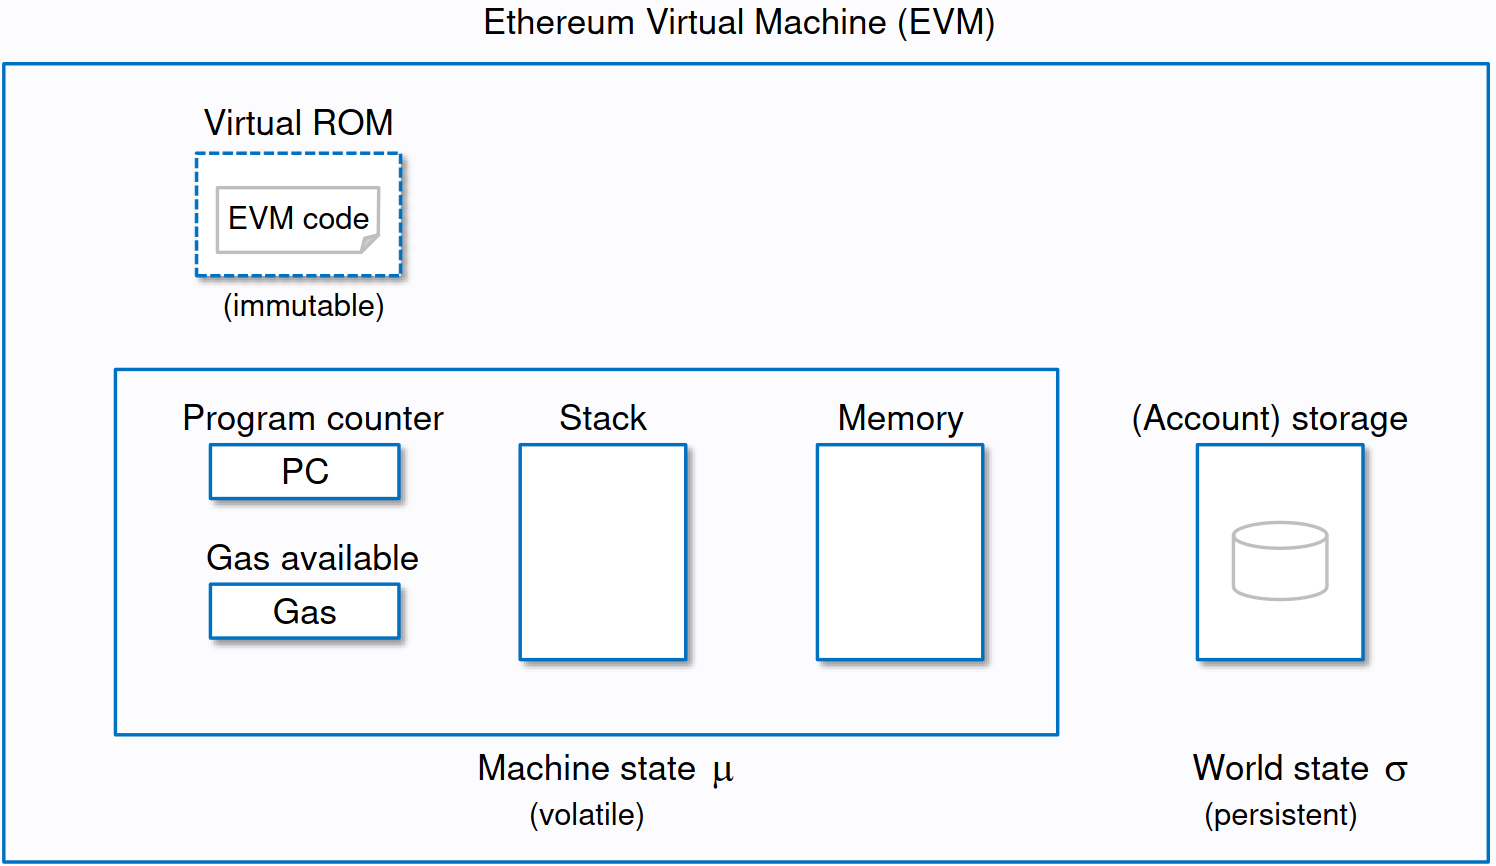
\includegraphics[width=1\columnwidth]{ch2/evm.png}
   \captionsource{Diagram of EVM architecture}
   {Diagram of EVM architecture as described in Ethereum Yellow Paper \cite{ethereum_yellow_paper}.
   }{\url{https://takenobu-hs.github.io/downloads/ethereum_evm_illustrated.pdf}}
   \label{fig:evm}
\end{figure}

% ----------------------------------------------------------------------------- DONE

\subsection{Currency}
\label{subsec:currency_and_issuance}


The Ethereum white paper \cite{ethereum_white_paper} describes the currency and issuance as follows:




\begin{quote}
  \textit{The Ethereum network includes its own built-in currency, ether, which serves the dual purpose of providing a primary
      liquidity layer to allow for efficient exchange between various types of digital assets and, more importantly, of providing a
      mechanism for paying transaction fees.}




  \textit{(Vitalik Buterin, Ethereum White Paper, 2014)}
\end{quote}




The currency of Ethereum is called \textit{ether} and is used to pay for transaction fees and computational services. The smallest unit
of ether is called \textit{wei}. The denomination of ether is as follows:




\begin{table}[H]
  \centering
  \begin{tabular}{|l|l|l|}
      \hline
      % merge 3 cells in the first line
      \multicolumn{3}{|c|}{\textbf{Denonimation of Ether}}                 \\ \hline
      \textbf{Unit name} & \textbf{Value of Wei} & \textbf{Value of Ether} \\ \hline
      Wei (wei)          & $1$                   & $1\times10^{-18}$       \\ \hline
      $K$wei (babbage)   & $10^{3}$              & $1\times10^{-15}$       \\ \hline
      $M$wei (lovelace)  & $10^{6}$              & $1\times10^{-12}$       \\ \hline
      $G$wei (shannon)   & $10^{9}$              & $1\times10^{-5}$        \\ \hline
      $T$wei (szabo)     & $10^{12}$             & $1\times10^{-5}$        \\ \hline
      $P$wei (finney)    & $10^{15}$             & $1\times10^{-3}$        \\ \hline
      ether (buterin)    & $10^{18}$             & $1$                     \\ \hline
  \end{tabular}
  \caption{Ether denominations.}
  \label{tab:ether_denominations}
\end{table}




The wei denomination is designed for an internal representation of the data. The wei unit is used in most cases, and the values
are displayed in either denomination or other denominations in the user interface. It means the user does not need to
know the wei denomination to use the Ethereum network. Therefore, users interact with the Ethereum network using the ether denomination.


The Ethereum network has a fixed supply of ether, and the issuance of ether
is the way to create new ether. This process goes through mining\footnote{Mining is the process of adding new blocks to the blockchain.},
which involves solving a computationally difficult puzzle by miners\footnote{Miners are the nodes that participate in the mining process. They are
called miners because of the analogy with traditional mining, where miners are rewarded with gold for their work.}.
Miners contribute their computational power to the network and are rewarded with ether by successfully mining a block by solving the puzzle.
Note that the issuance of ether through mining has several purposes. First, it incentivizes miners to secure the network by validating transactions
and maintaining the integrity of the blockchain. Second, it ensures an adequate supply of ether, allowing actors to perform transactions and interact
with decentralized applications on the Ethereum network.




One core of the principles of Ethereum is the concept of \textit{Proof of Work} (PoW) consensus mechanism, where a fixed amount of ether is locked
for each successful block mined. Nevertheless, Ethereum plans to switch to a \textit{Proof of Stake} (PoS) consensus mechanism, known as
Ethereum 2.0. With the PoS consensus mechanism, the issuance of ether will occur through staking, where actors lock their ether as collateral to
participate in the consensus mechanism and receive rewards for their work. The Ethereum Foundation \cite{eth_proofofstake} explains the switch
to PoS as follows:


\begin{quote}
   \textit{The Ethereum network began by using a consensus mechanism that involved Proof-of-work (PoW). This allowed the nodes of the Ethereum network to agree on the state of all information recorded on the Ethereum blockchain
   and prevented certain kinds of economic attacks. However, Ethereum switched off proof-of-work in 2022 and started using proof-of-stake instead.}


   \textit{(Ethereum Foundation)}
\end{quote}


The issuance of new ether plays a crucial role in the functioning of the Ethereum network, providing necessary incentives for miners and ensuring
availability of ether for various transactions and interactions on the platform.



% ----------------------------------------------------------------------------- DONE

\subsection{Gas}
\label{subsec:gas}


Gas is essential to the Ethereum network. The Ethereum white paper \cite{ethereum_white_paper} describes gas as follows:


\begin{quote}
   \textit{In order to prevent accidental or hostile infinite loops or other computational wastage in code, each transaction is
       required to set a limit to how many computational steps of code execution it can use. The fundamental unit of computation is "gas";
       usually, a computational step costs 1 gas, but some operations cost higher amounts of gas because they are more computationally expensive,
       or increase the amount of data that must be stored as part of the state.}


   \textit{(Vitalik Buterin, Ethereum White Paper, 2014)}
\end{quote}


Gas represents the unit that measures the computational effort required to execute operations or run programs in the Ethereum network.
Each transaction requires a certain amount of resources to be executed. Thus each transaction requires a fee. Gas refers to the fee required to
execute a transaction or a message in Ethereum even if the transaction succeeds or fails.


\begin{figure}[H]
   \centering
   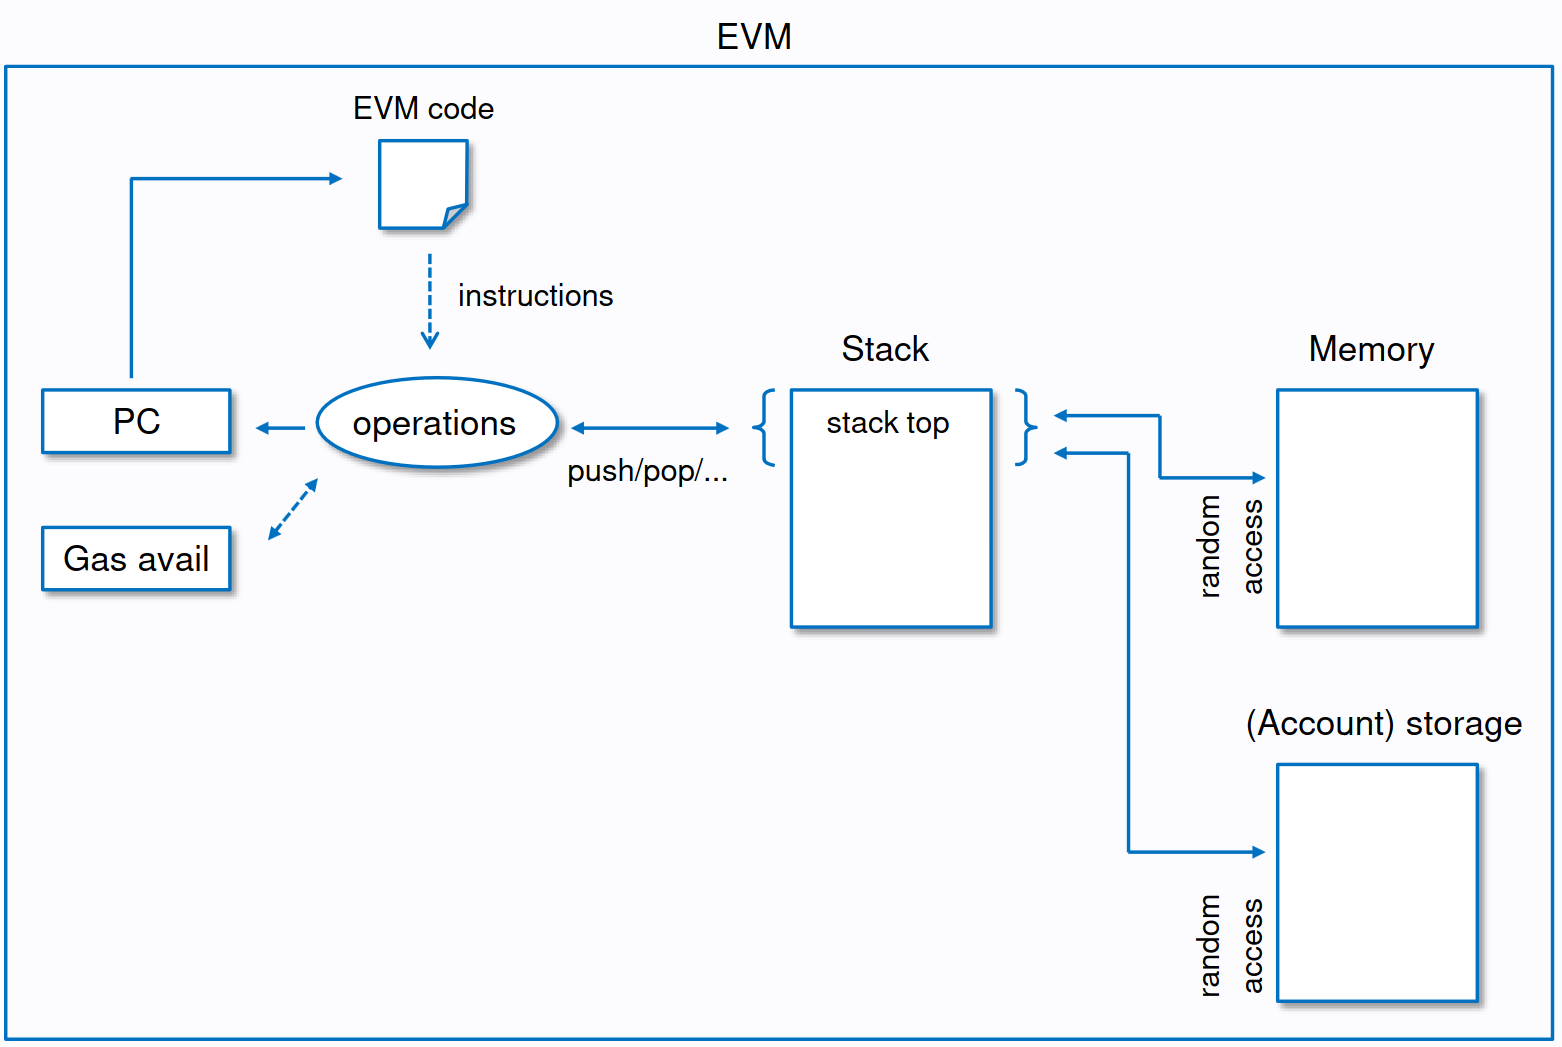
\includegraphics[width=0.8\textwidth]{ch2/gas.png}
   \captionsource{Diagram of execution model }
   {Diagram of execution model as described in Ethereum Yellow Paper \cite{ethereum_yellow_paper}.}
   {\url{https://takenobu-hs.github.io/downloads/ethereum_evm_illustrated.pdf}}
   \label{fig:gas}
\end{figure}


Figure \ref{fig:gas} above shows the execution model of the Ethereum Virtual Machine, where the gas is used to pay for the execution of the code. Another
value is \texttt{GASLIMIT}. This value is the maximum amount of gas used on a transaction. For example, some complicated transactions may require more gas than the
default gas limit. If the gas limit is too low, the transaction will fail, and the gas will be consumed. Standard transactions have a gas limit of 21,000 gas.


% ----------------------------------------------------------------------------- DONE

\subsection{Fees}
\label{subsec:fees}


As in Bitcoin, the fees are a crucial part of the Ethereum network because they prevent the network from being overloaded by computations. The difference between Bitcoin 
and Ethereum is that in Bitcoin, the fees are paid per byte of data, whereas in Ethereum, the fees are paid per computational step. As mentioned in the previous section 
\ref{subsec:gas}, the gas is used to prevent infinite loops or other computational wastage in code. The \texttt{STARTGAS} (see section \ref{subsec:messages_and_transactions}) 
value is the maximum number of computational steps the transaction execution is allowed to take. Every transaction requires a limit of gas to prevent infinite loops. 
Each computational step costs a certain amount of gas, typically one gas. However, some operations cost more due to their computational complexity or due to storage space.


The transaction fee is an integral part of each transaction and serves as a deterrent against spam attacks. Transactions requiring more resources will incur higher fees compared 
to those with fewer resources, making the fee proportional to the transaction size. The calculation of the transaction fee is demonstrated by the equation below.


\begin{equation}
   \label{eq:transaction_fee}
   \text{Transaction Fee} = \texttt{STARTGAS} \times \texttt{GASPRICE}
\end{equation}


One advantage of decoupling the execution cost from a specific currency, such as setting the cost of a computation step to three wei, is separating transaction 
execution cost from the fluctuations in Ether's value compared to fiat currencies. For example, if the price of Ether significantly rises relative to a currency like the 
dollar, a fixed price per computational step could become unaffordable. To address this concern, the \texttt{GASPRICE} (see section \ref{subsec:messages_and_transactions}) 
is used to set the price of gas in Ether, ensuring a consistent amount of gas consumed by the transaction while allowing for adjustments in the overall gas price.

% ----------------------------------------------------------------------------- DONE


\section{Solidity, a high-level language for Ethereum}
\label{sec:ch2_solidity}


To interact with the Ethereum network, we need to write smart contracts. For this purpose, we use Solidity, a high-level language for
implementing smart contracts. Solidity is a statically typed language that supports inheritance, libraries, and complex user-defined types
, among other features.
From the official documentation \cite{ethereum_solidity_doc}, Ethereum foundation describes Solidity as follows:


\begin{quote}
   \textit{Solidity is an object-oriented, high-level language for implementing smart contracts. Smart contracts are programs that govern the behavior of accounts within the Ethereum state.
       Solidity is a curly-bracket language designed to target the Ethereum Virtual Machine (EVM). It is influenced by C++, Python, and JavaScript.You can find more details about which languages Solidity has been inspired by in the language influences section.}


   \textit{(Ethereum Foundation)}
\end{quote}



The Solidity compiler, known as \textit{solc}, is responsible for compiling Solidity code into bytecode that can be executed on the Ethereum Virtual Machine (EVM). 
Developed in C++, the Solidity compiler is licensed under the GNU Lesser General Public License v3.0 (LGPL). It offers both command-line utility and library 
functionalities, providing flexibility in its usage.

In summary, all smart contracts for our project are written in Solidity and compiled into EVM-executable bytecode. The upcoming sections will delve into the Solidity 
language and discuss the fundamental structure necessary to understand how we implemented the smart contracts in our project.


% ----------------------------------------------------------------------------- DONE

\subsection{State Variables}

State variables in Solidity serve as a contract's persistent data stored on the blockchain, retaining their values throughout multiple function calls. These 
variables define the properties and attributes of a contract and are accessible to all functions within it.

To declare a state variable in Solidity, we specify its type, visibility, and optional modifiers. Solidity offers a range of data types, including integers, booleans, 
strings, arrays, structs, and user-defined types. These data types enable the representation and manipulation of different kinds of data within the smart contract.

\begin{listing}[!ht]
    \begin{minted}[]{solidity}
// SPDX-License-Identifier: GPL-3.0
pragma solidity ^0.8.0;

contract SimpleStorage {
    uint256 public storedData;
    string public name = "SimpleStorage";

    function set(uint256 x) public {
        storedData = x;
    }

    function get() public view returns (uint256) {
        return storedData;
    }
}
    \end{minted}
    \caption{Example of a contract with a state variable.}
    \label{lst:state_variable}
\end{listing}

In the Listing \ref{lst:state_variable}, the contract \texttt{SimpleStorage} has a state variable \texttt{storedData} of type \texttt{uint256}.
By utilizing state variables, Solidity provides a powerful mechanism for managing and preserving the state of contracts on the blockchain, facilitating the development of 
robust and feature-rich decentralized applications.

% ----------------------------------------------------------------------------- DONE

\subsection{Functions}




Functions in Solidity play a crucial role in implementing the logic of a contract and are similar to functions in other programming languages. They can 
be declared with different visibilities, including \texttt{external}, \texttt{public}, \texttt{internal}, or \texttt{private}. The default visibility is \texttt{public}.


\begin{listing}[!ht]
    \begin{minted}[]{solidity}
// SPDX-License-Identifier: GPL-3.0
pragma solidity ^0.8.0;

contract MySimpleFunction {
    constructor() {
        // constructor
    }

    function mint(address account, uint256 amount) public onlyOwner {
        _mint(account, amount);
    }

    function decimals() public view virtual override returns (uint8) {
        return 2;
    }

}
    \end{minted}
    \caption{Example of a contract with a function.}
    \label{lst:function}
\end{listing}

In the provided Listing \ref{lst:function}, we show a contract named \texttt{MySimpleFunction} that implements two functions: \texttt{mint} and \texttt{decimals}.
The \texttt{mint} function is declared as \texttt{public}, allowing anyone to call it. It is responsible for minting tokens by invoking the \texttt{\_mint} function.
On the other hand, the \texttt{decimals} function is declared as \texttt{public view}, indicating that anyone can call it and only reads data from the contract without
modifying the state. In this case, the \texttt{decimals} function returns the number of decimals for the token without requiring a transaction and, therefore, is free of
charge of gas.

% ----------------------------------------------------------------------------- DONE

\subsection{Function Modifiers}

\begin{listing}[!ht]
    \begin{minted}[]{solidity}
// SPDX-License-Identifier: GPL-3.0
pragma solidity ^0.8.0;

contract MyToken{
    address public owner;
    
    modifier onlyOwner() {
        require(msg.sender == owner, "Only owner can call this function.");
        _;
    }

    constructor() {
        owner = msg.sender;
    }

    function transferOwnership(address newOwner) public onlyOwner {
        owner = newOwner;
    }
}
    \end{minted}
    \caption{Example of a contract with a function modifier.}
    \label{lst:modifier}
\end{listing}


In the Listing \ref{lst:modifier}, the contract \texttt{MyToken} has a function modifier \texttt{onlyOwner}. The function modifier \texttt{onlyOwner} restricts
access to certain functions. In this case, only the owner of the contract can call the function \texttt{transferOwnership}.
The variable \texttt{msg.sender} is a global variable that contains the address of the sender of the message. The underscore (\texttt{\_}) in the function modifier
indicates where the function body will be executed.


% ----------------------------------------------------------------------------- DONE

\subsection{Events}

Events are used to notify external applications about the occurrence of a specific event. This allows direct interaction with EVM logs.
Events are an essential part of the Ethereum ecosystem because they allow to interact with smart contracts in a decentralized way, for example
dApps (Decentralized Applications) and Oracles\footnote{Oracles are third-party services that provide smart contracts with external information.}.

\begin{listing}[!ht]
   \begin{minted}[]{solidity}
// SPDX-License-Identifier: GPL-3.0
pragma solidity ^0.8.0;


contract MyTokenAction{
   event Transfer(address indexed from, address indexed to, uint256 value);


   function transfer(address _to, uint256 _value) public returns (bool success) {
       emit Transfer(msg.sender, _to, _value);
       return true;
   }
}
   \end{minted}
   \caption{Example of a contract with an event.}
   \label{lst:event}
\end{listing}


In Listing \ref{lst:event}, the contract \texttt{MyTokenAction} shows the usage of an event called \texttt{Transfer}. The \texttt{Transfer} event serves to notify external applications about the transfer of tokens. The \texttt{transfer} function, responsible for transferring tokens from one address to another, emits the
\texttt{Transfer} event after completing the token transfer. The \texttt{emit} keyword triggers the event, providing the necessary arguments.

% ----------------------------------------------------------------------------- DONE

\subsection{Structs}

Structs in Solidity serve as a mechanism for defining custom data types. They are similar to structs in C or C++ and are utilized to group variables, creating a cohesive 
data structure. As a result, structs are particularly valuable for organizing and storing data within smart contracts.


\begin{listing}[!ht]
    \begin{minted}[]{solidity}
// SPDX-License-Identifier: GPL-3.0
pragma solidity ^0.8.0;

contract Orderbook {

    struct Order {
        uint amount;
        uint price;
        uint timestamp;
        address trader;
        bytes2 status;
    }
}
    \end{minted}
    \caption{Example of a contract with a struct.}
    \label{lst:struct}
\end{listing}

In Listing \ref{lst:struct}, we present the contract \texttt{Orderbook}, which incorporates a struct named \texttt{Order}. 
This struct is responsible for storing order-related data. Within the \texttt{Order} struct, several properties are defined, including \texttt{amount}, \texttt{price}, 
\texttt{timestamp}, \texttt{trader}, and \texttt{status}. By utilizing the \texttt{Order} struct, the contract can effectively store and manage order data within the 
order book.

% ----------------------------------------------------------------------------- DONE

\subsection{Common Data Types in Solidity}

Solidity supports various data types that allow developers to define and manipulate variables within smart contracts. Here are some common data types used in Solidity:

\begin{itemize}
   \item \textbf{Integers}: Solidity provides signed and unsigned integer types with different bit sizes. For example, \texttt{uint} represents an unsigned integer, and \texttt{int} represents a signed integer. You can specify the number of bits by appending the number, such as \texttt{uint256} or \texttt{int8}.


   \item \textbf{Booleans}: Solidity includes a \texttt{bool} type that can store either \texttt{true} or \texttt{false}.


   \item \textbf{Bytes}: Solidity provides a \texttt{bytes} type that can be used to store byte arrays. For example, \texttt{bytes32} represents a byte array of 32 bytes. The \texttt{bytes} type is similar to the \texttt{string} type, but it is not UTF-8 encoded and does not support string operations.


   \item \textbf{Address}: The \texttt{address} type represents a 20-byte Ethereum address. It can store Ethereum and contract addresses and provides various member functions to interact with.


   \item \textbf{Strings}: Solidity supports string types (\texttt{string}) for storing and manipulating variable-length text data.


   \item \textbf{Arrays}: Solidity allows the declaration of fixed-size and dynamic arrays. Fixed-size arrays have a predefined length, such as \texttt{uint[5]} for an array of five unsigned integers. Dynamic arrays can have a variable length, such as \texttt{uint[]} for an array of unsigned integers.


   \item \textbf{Mappings}: Solidity provides mappings and key-value stores that associate values with unique keys. Mappings can be used to implement data storage and retrieval efficiently. For example, \texttt{mapping(address => uint)} represents a mapping that associates unsigned integers with addresses.


   \item \textbf{Enums} allows us to define a set of named constants. Each constant has an associated integer value. Enums help define states or options within a contract.


   \item \textbf{Function Types}: Solidity supports function types, which enable us to declare variables or parameters that can store or refer to functions. Function types help implement callback mechanisms or pass functions as arguments.


\end{itemize}

These data types have been selected based on their relevance to our project and are commonly used to develop smart contracts. Using these data types in our project ensures efficient and secure data handling within the contract.
It is important to note that Solidity offers a broader range of data types beyond those mentioned in this list. The official Solidity documentation \cite{ethereum_solidity_doc} refers to a comprehensive understanding of all 
available data types and their specific use cases.

% ----------------------------------------------------------------------------- DONE

\subsection{UML Diagram for Solidity Code}

Unified Modeling Language (UML) diagrams are graphical representations that visualize the structure and relationships of various elements
in software systems. While UML diagrams are commonly used for object-oriented programming languages, they can also be adapted to represent
Solidity code. This project uses UML diagrams to represent the structure and relationships between our Token and exchange contracts.
To create UML diagrams in \LaTeX, we use the \texttt{tikz-uml} package. This package provides a set of macros for creating UML sequence diagrams, class diagrams, 
and other UML diagram types.


Here is an example of how to represent a UML class diagram for Solidity code using the \texttt{tikz-uml} package:


\begin{figure}[H]
   \centering
   \begin{tikzpicture}[scale=0.8, transform shape]
       \begin{umlpackage}{MyToken}
           \umlclass{MyToken}{}{
               + owner: address \\
               \umlstatic{-- onlyOwner() : modifier} \\
               \umlstatic{+ transferOwnership(newOwner: address) : void}
           }


           \umlclass[x=3,y=-5]{address}{}{}


           \umlaggreg[mult1=1,pos1=0.2,mult2=1,pos2=0.8]{MyToken}{address}
           \umluniassoc[arg1=owner,arg2=address,pos=0.5]{MyToken}{address}


           \umlnote[x=0,y=-7,width=7.5cm]{MyToken}{\textbf{Note:} The \texttt{onlyOwner()} function is a modifier in the \texttt{MyToken} contract that ensures the owner of the contract can only execute some functions.}
       \end{umlpackage}
   \end{tikzpicture}
   \caption{UML Class Diagram for Solidity Code}
   \label{fig:uml_diagram}
\end{figure}

Figure \ref{fig:uml_diagram} shows a UML class diagram for the Solidity code presented in the Listing \ref{lst:function}. The \texttt{tikz-uml} package provides macros
for creating UML classes, sequences, and other UML diagram types.

\begin{figure}[H]
    \centering
    \begin{tikzpicture}[thick]
        \begin{umlseqdiag}
            % Participant: Owner
            \umlactor[class=Owner,,fill=white!0]{Alice}

            % Participant: Contract
            \umldatabase[class=Contract,fill=white!0,x=5]{MyToken}

            % Alice calls transferOwnership(Bob)
            \begin{umlcall}[op={transferOwnership(Bob)}, return=emit OwnershipTransferred, draw=SkyBlue, fill=SkyBlue!20, dt=5]{Alice}{MyToken}
                % Contract calls onlyOwner()
                \begin{umlcallself}[op={onlyOwner()}, fill=ForestGreen!20, draw=ForestGreen, return=true]{MyToken}
                \end{umlcallself}
            \end{umlcall}

            % Alice attempts to transfer ownership again, but it fails
            \begin{umlcall}[op={transferOwnership(Alice)},return=revert, draw=SkyBlue,fill=SkyBlue!20, dt=5]{Alice}{MyToken}
                % Contract calls onlyOwner()
                \begin{umlcallself}[op={onlyOwner()}, fill=ForestGreen!20, draw=ForestGreen, return=false]{MyToken}
                \end{umlcallself}
            \end{umlcall}

            % Transaction indicator
            \filldraw[draw=SkyBlue,fill=SkyBlue!20] (1.2,-5) circle (.2);
            \node at (0,-5) {Transaction};

            % Call indicator
            \filldraw[draw=ForestGreen,fill=ForestGreen!20] (3,-5) circle (.2);
            \node at (3.6,-5) {Call};
        \end{umlseqdiag}
    \end{tikzpicture}
    \caption{UML Sequence Diagram for presenting the function \texttt{transferOwnership}.}
    \label{fig:uml_sequence_diagram}
\end{figure}



Figure \ref{fig:uml_sequence_diagram} illustrates a UML sequence diagram corresponding to the Solidity code presented in Listing \ref{lst:function}. The diagram captures 
the sequence of interactions between the involved actors, namely Alice and Bob, and the contract's functions.
In the diagram, Alice initiates the process by calling the function \texttt{transferOwnership}, which transfers her ownership to Bob. This function internally invokes the 
\texttt{onlyOwner} modifier to verify whether the caller is the contract owner. If the caller is not the owner, the \texttt{onlyOwner} function reverts the transaction, 
preventing the transfer of ownership. The transaction is reverted in this scenario because Alice is not the contract owner since she has already transferred her ownership to Bob.
The diagram distinguishes between transactions and calls using different colors. Blue circles represent transactions, while calls are depicted with green circles.
This UML sequence diagram provides a visual representation of the interactions and control flow within the contract, aiding in understanding its functionality and behavior.


% ----------------------------------------------------------------------------- DONE

\section{Ethereum Token Standards}
\label{sec:ch2_ethereum_token_standards}

In blockchain technology and cryptocurrencies, a token is essential in allowing more possibilities and use cases of decentralized
applications and ecosystems. A token represents a digital asset that can be compared in various forms of value, such as money, loyalty points, gold certificates, and more.
To enable interoperability, consistency, and compatibility between different tokens, the Ethereum community has created a set of token standards.
These standards are called Ethereum Request for Comments (ERC). The ERC standards are Ethereum Improvement Proposals (EIP) that define a set of rules
that a token must implement to be ERC-compliant.


This section focuses on presenting token standards with a particular focus on the Ethereum blockchain. The Ethereum platform is
known for its innovative contract capabilities and therefore is a pioneer in creating token standards through EIPs.
Their proposals define the specifications and norms that a token must follow, ensuring uniformity and facilitating the integration
of tokens in different applications.


In the following subsections, we describe the concept of a token, providing a general overview of the token standards. Then, we present
the Ethereum Improvement Proposals created to define the token standards. Finally, we explore some of the cryptocurrency ecosystem's most popular
token standards and innovations.


% ----------------------------------------------------------------------------- DONE

\subsection{What is a Token ?}

A token digitally represents an asset or utility within a decentralized network. It is often created and issued by
a smart contract, a self-executing contract of rules with predefined conditions on the blockchain. We can compare a token
to a physical token in the real world, where a token can represent ownership rights or access to a service. In the Ethereum Whitepaper
\cite{ethereum_white_paper}, Vitalik Buterin defines a token as follows:

\begin{quote}
   \textit{On-blockchain token systems have many applications ranging from sub-currencies representing assets such as USD or gold to
       company stocks, individual tokens representing smart property, secure unforgeable coupons, and even token systems with no ties to
       conventional value at all, used as point systems for incentivization.}


   \textit{(Vitalik Buterin, Ethereum Whitepaper)}
\end{quote}


We can illustrate the concept of a token with an example. First, let us consider an analogy for an IT Security convention like the DEF CON
\footnote{DEFCON is one of the world's largest hacker conventions, held annually in Las Vegas, Nevada.} convention. Imagine we attend
the DEFCON convention, and as we enter the convention, we receive a special badge that gives us certain privileges. This badge
is similar to a token because it allows us to access certain convention areas, participate in exclusive events
, and receive certain benefits. However, in this case, the badge represents a value within the DEFCON convention, enabling us to engage
in certain activities.

We can cite some examples of tokens such as Aragon (ANT)\footnote{Aragon Token: \url{https://aragon.org/}} and Basic Attention Token (BAT)\footnote{Basic Attention Token: \url{https://basicattentiontoken.org/}}.
Aragon provides governance rights within the Aragon Network. Holding Aragon tokens gives the holder the right to vote on certain
decision-making processes and influence the direction of the project.

From a business perspective, a token can offer the company a new opportunity to issue shares, securities, or their own
currency, allowing them to take control of their finances. In addition, companies can use tokens to get exclusive access to certain services
or products within their ecosystem. For example, many companies use tokens to raise project funds through Initial Coin Offerings (ICO)\footnote{ICO: \url{https://en.wikipedia.org/wiki/Initial_coin_offering}}.
An ICO is a fundraising mechanism in which new projects sell their underlying crypto tokens in exchange for bitcoin and ether. It is
similar to an Initial Public Offering (IPO)\footnote{IPO: \url{https://en.wikipedia.org/wiki/Initial_public_offering}},
 in which investors purchase company shares. Creating a cryptocurrency token for
international settlements allows companies to avoid intermediaries and reduce costs and transaction time. However, regulatory compliance is
critical for companies that want to issue tokens with specific characteristics.


% ----------------------------------------------------------------------------- DONE

\subsection{Ethereum Improvement Proposals}
\label{subsec:eip}

The Ethereum Improvement Proposals (EIP) are crucial in defining standards and guidelines for token creation and implementation on the Ethereum
platform. EIPs are formal documents submitted by Ethereum community members (like developers and researchers) to propose improvements
, new features, and changes to the Ethereum protocol.


Regarding token standards, the Ethereum Requests for Comments (ERC) are EIPs that define a set of rules that a token must implement on the Ethereum
platform to adhere to the standard. It ensures that the tokens created are compatible and interoperable among different projects and applications.
ERCs are defined as a significant contribution to the Ethereum ecosystem and are widely used by the community. The official documentation
for ERCs can be found on the Ethereum GitHub repository\footnote{Ethereum GitHub repository: \url{https://github.com/ethereum/EIPs}}.
The ERC20 is by far the most popular token standard for fungible tokens\footnote{Fungible tokens are interchangeable and can be replaced by another token.},
offering consistency and integration for developers. In addition, ERC20 can represent any digital asset, such as cryptocurrencies, loyalty points, and gold certificates.


In addition to the ERC20, other token standards are widely used in the Ethereum ecosystem. We can cite notable token standards
such as the ERC721, introducing non-fungible tokens (NFTs)\footnote{Non-fungible tokens are unique and indivisible tokens that another token cannot replace.}
, which are unique and indivisible digital assets. NFTs are widespread in gaming, art, and collectibles, enabling
verifiable digital ownership and scarcity.


There are a lot of other token standards that are widely used in the Ethereum ecosystem. We can cite some examples, such as the ERC777 and ERC1155.
Ethereum Improvement Proposals and token standards have significantly contributed to the Ethereum ecosystem's growth and development, enabling
innovation, facilitating token creation, and diverse, decentralized applications on the Ethereum blockchain.


% ----------------------------------------------------------------------------- DONE

\subsection{Token standards}

As explained in the previous section \ref{subsec:eip}, the most approved token standard is the ERC20 which we describe more in detail in the section \ref{sec:ch2_erc20}.
Many other token standards are designed from the ERC20 for (1) suggesting improvements, (2) adding new features, (3) solving problems, or (4) proposing new functionalities.
Some proposals define entirely new token standards, such as the ERC777. The table \ref{tab:token_standards} shows some of the most popular token standards derived from the ERC20.

\begin{table}[h]
   \rowcolors{1}{gray!15}{white} % Set row colors, starting from the first row
   \begin{tabular}{|c|p{5cm}|p{3cm}|p{2cm}|}
       \hline
       \rowcolor{gray!50} % Set header row color
       \textbf{Token Standard} & \textbf{Description}                                                                                                                          & \textbf{Author}                                    & \textbf{Date} \\
       \hline
       ERC-20                  & The standard for fungible tokens on the Ethereum blockchain, ensuring interoperability and ease of integration.                               & Fabian Vogelsteller and Vitalik Buterin            & November 2015 \\
       \hline
       ERC-223 (Draft)         & An improvement over ERC-20, introducing enhanced security features and efficiency, including the ability to reject incoming token transfers.  & Dexaran                                            & March 2017    \\
       \hline
       ERC-777                 & A more advanced token standard that fixes some of the issues with ERC-20, including the sending mechanism for regular accounts and contracts. & Jordi Baylina, Jacques Dafflon, and Thomas Shababi & November 2017 \\
       \hline
       ERC-827                 & An extension of ERC-20, providing additional functionalities like approving token transfers on behalf of the token holder.                    & Joseph Chow                                        & January 2018  \\
       \hline
   \end{tabular}
   \caption{List of some  EIPs token standards derived from the ERC20.}
   \label{tab:token_standards}
\end{table}

Table \ref{tab:token_standards} provides an overview of token standards, illustrating that the ERC20 token standard was the first to be established in November 2015.
Subsequently, other token standards have emerged, building upon the foundation set by ERC20. It is important to note that the table represents a selection and is not exhaustive. To explore the complete documentation and comprehensive lists of token standards, one can visit the official website of Ethereum Improvement Proposals (EIPs)
\cite{ethereum_eip}. The EIPs website is a valuable resource for the community, providing access to drafts and proposals open for review and discussion.

% ----------------------------------------------------------------------------- DONE

\section{ERC20 Token Standard}
\label{sec:ch2_erc20}

This section introduces the importance of selecting appropriate token standards for our settlement solution. Tokens serve as a medium of exchange and can represent any digital asset
such as cryptocurrencies, enabling seamless and secure transactions. With numerous tokens at our disposal, the ERC20 token standard is the most popular and widely adopted choice for
fungible tokens because of its simplicity and interoperability. We provide an overview of the ERC20 token standard, explaining its functionalities and features.

% -----------------------------------------------------------------------------

\subsection{Overview of ERC20}

The ERC20 token standard stands for Ethereum Request for Comments 20 and has been proposed by Fabian Vogelsteller and Vitalik Buterin in 19\textsuperscript{th} November 2015 \cite{eth_erc20}.
It introduces a standardized interface for fungible tokens on the Ethereum blockchain, ensuring interoperability and ease of integration among different projects. ERC20 tokens are
designed to be interchangeable and can be replaced by any other token of the same type and exchanged on a one-to-one basis. This particular feature called fungibility makes ERC20
tokens suitable for representing currencies, digital assets, and other financial instruments where uniformity and interchangeability are vital. This allows developers to
create decentralized applications (DApps) that can interact with any ERC20 token without implementing custom code for each token. The ERC20 interface specifies a set of functions
called ERC20 methods that the token contract must implement. The methods allow actors to transfer their tokens to other addresses, get the current token balance of an address, and approve
the transfer of tokens from one address to another. The following code snippet shows the ERC20 interface in Solidity from the EIP-20 \cite{eth_erc20}.

\begin{listing}[!ht]
   \begin{minted}[]{solidity}
interface IERC20 {
   function name() external view returns (string memory);
   function symbol() external view returns (string memory);
   function decimals() external view returns (uint8);
   function totalSupply() external view returns (uint256);
   function balanceOf(address account) external view returns (uint256);
   function transfer(address recipient, uint256 amount) external returns (bool);
   function transferFrom(address sender, address recipient, uint256 amount) external returns (bool);
   function allowance(address owner, address spender) external view returns (uint256);
   function approve(address spender, uint256 amount) external returns (bool);
   event Transfer(address indexed from, address indexed to, uint256 value);
   event Approval(address indexed owner, address indexed spender, uint256 value);
}
   \end{minted}
   \caption{ERC20 interface in Solidity.}
   \label{lst:erc20_interface}
\end{listing}


The listing \ref{lst:erc20_interface} shows the ERC20 interface in Solidity representing nine functions and two events. The functions are described as follows:


\begin{itemize}
   \item \mintinline{solidity}|name()|: Returns the token's name as the name suggests. E.g. the name of \textit{Universal Export Token} is \texttt{Universal Export Token}.
   \item \mintinline{solidity}|symbol()|: Returns the token's symbol, usually a shorter name version. E.g. the symbol of \textit{Universal Export Token} is \texttt{UET}.
   \item \mintinline{solidity}|decimals()|: Returns the number of decimals used to get its user representation. For example if \texttt{decimals} equals $2$, a balance of 12345 tokens should be displayed to a user as $123.45$.
   \item \mintinline{solidity}|totalSupply()|: Returns the total token supply.
   \item \mintinline{solidity}|balanceOf(address)|: Returns the token balance of a given address.
   \item \mintinline{solidity}|transfer(address, amount)|: Transfers a specified amount of tokens from the sender's address to the recipient's address. The function returns a boolean
         value indicating whether the operation was successful and must fire the \mintinline{solidity}|Transfer| event. The return value of 0 indicates that the transfer was successful.
   \item \mintinline{solidity}|transferFrom(from, to, amount)|: Transfers a specified amount of tokens from one address to another. The function returns a boolean value
         indicating whether the operation was successful and must fire the \mintinline{solidity}|Transfer| event. This method is used for a withdrawal workflow,
         meaning that a user can transfer tokens on behalf of another user (e.g. a decentralized exchange) with charge fees.
   \item \mintinline{solidity}|allowance(owner, spender)|: Returns the current allowance of a spender for a given owner. The allowance is the maximum amount of tokens a spender can spend on behalf of the owner.
   \item \mintinline{solidity}|approve(spender, amount)|: Allows a spender to transfer a specified amount of tokens on behalf of the token owner.
   \item \mintinline{solidity}|Transfer(address, address, amount)|: Emitted when tokens are transferred from one address to another. The event is triggered when tokens are transferred by the \mintinline{solidity}|transfer| and \mintinline{solidity}|transferFrom| functions.
   \item \mintinline{solidity}|Approval(address, address, amount)|: Emitted when the allowance of a spender for an owner is set by the \mintinline{solidity}|approve| function. The event is triggered when the allowance is set by the \mintinline{solidity}|approve| function.
\end{itemize}

All balances and amount parameters are represented on 256 bits unsigned integers, thus the maximum amount of tokens that can be handled is $2^{256} - 1$. The point is to make that some functions are declared as \texttt{view} functions
like \mintinline{solidity}|name()|, \mintinline{solidity}|symbol()|, etc. It indicates that the function does not modify the state of the contract and does not consume any gas. The \texttt{view} functions are free to call and do not require gas.
It can be compared to a getter function in object-oriented programming that returns a private variable's value. Another critical point is the \mintinline{solidity}|decimal()| function. When working
with tokens, we usually work with a very small amount, representing a fraction of a token. For example, if one owns 4 UET tokens, transferring 3.49 UET to another address may be necessary, and keeping 0.51 UET in the sender's address. The EVM does not support floating point numbers, so Solidity allows us to define the integer number values of the token that should be displayed as a fraction of a token.
It can be a problem because if one wants to transfer 3.49 UET, the number of tokens to transfer can be only 3 UET or 4 UET.

To solve this problem, ERC20 tokens include the \mintinline{solidity}|decimals()| function that returns the number of decimals used to get its user representation. For example, if \mintinline{solidity}|decimals()| equals $2$,
it is possible to transfer 3.49 UET by transferring 349 UET and keeping 51 UET in the sender's address. It is important to note that the \mintinline{solidity}|decimals()| function is only used for display purposes
and does not affect the arithmetic of the token. A decimal value of 2 is usually common in many other ERC20 tokens. It means when we mint or transfer tokens, we work with a value of :

\begin{center}
    \begin{equation}
        \centering
        \text{value} = \text{UET} \times 10^{\text{decimals}}
    \end{equation}
    \label{eq:decimals}
 \end{center}
 
 
 For example, if we want to mint 1000 UET, we mint $1000 \times 10^2 = 100000$ UET, the same process for transferring tokens. However, some tokens
 like Ether have a decimal value of 18, which means that when we transfer 1 Ether, we transfer $1 \times 10^{18} = 1000000000000000000$ Wei. Some others have a decimal value of 0,
 which means that when we transfer 1 token, we transfer $1 \times 10^0 = 1$ token. It can make sense for some tokens like a token representing a share of a company. It is not possible to transfer
 a fraction of a share. 

% ----------------------------------------------------------------------------- DONE

\subsection{Methods of the ERC20 interface}
\label{subsec:erc20_methods}


The \texttt{allowance} method enables an owner, such as Alice, to verify the number of tokens that a spender, such as Bob, is permitted to transfer on their behalf. This method takes two parameters: the owner's address and the spender's address. It returns the number of tokens the spender is authorized to spend on behalf of the owner.
Listing \ref{lst:openzeppelin_allowance} exemplifies the implementation of the \texttt{allowance} function in the OpenZeppelin library. Notably, this function is classified as a \texttt{view} function, indicating that it does not modify the state of the contract and does not consume any gas during execution.
The usage of the \texttt{virtual} keyword signifies that a child contract can override the function, offering flexibility for customization. Additionally, the \texttt{override} keyword indicates that the function overrides a corresponding function in the parent contract, ensuring the appropriate behavior and consistency within the contract hierarchy.


\begin{listing}[!ht]
   \begin{minted}[]{solidity}
/**
* @dev See {IERC20-allowance}.
*/
function allowance(address owner, address spender) public view virtual override returns (uint256) {
   return _allowances[owner][spender];
}
   \end{minted}
   \caption{OpenZeppelin implementation of the \texttt{allowance} function.}
   \label{lst:openzeppelin_allowance}
\end{listing}



The \texttt{approve} method enables an owner, such as Alice, to grant permission to a spender, such as Bob, to transfer a specific quantity of tokens on their behalf. By invoking this method, the owner sets the allowance for Bob to the designated value.
Listing \ref{lst:openzeppelin_approve} shows the implementation of the \texttt{approve} function in the OpenZeppelin library. 
This function provides a standardized and secure approach for granting token transfer permissions.

\begin{listing}[!ht]
    \begin{minted}[]{solidity}
/**
* @dev Sets `amount` as the allowance of `spender` over the `owner` s tokens.
*
* This internal function is equivalent to `approve`, and can be used to
* e.g. set automatic allowances for certain subsystems, etc.
*
* Emits an {Approval} event.
*
* Requirements:
*
* - `owner` cannot be the zero address.
* - `spender` cannot be the zero address.
*/
function _approve(address owner, address spender, uint256 amount) internal virtual {
    require(owner != address(0), "ERC20: approve from the zero address");
    require(spender != address(0), "ERC20: approve to the zero address");

    _allowances[owner][spender] = amount;
    emit Approval(owner, spender, amount);
}
    \end{minted}
    \caption{OpenZeppelin implementation of the \texttt{approve} function.}
    \label{lst:openzeppelin_approve}
\end{listing}

The implementation shown in Listing \ref{lst:openzeppelin_approve} includes two conditions on lines 15 and 16 that must be satisfied to execute the approval process. These checks ensure that both the owner and the spender addresses are not the zero addresses.
The zero address, denoted as \texttt{address(0)}, holds special significance in Ethereum. It represents the absence of an address and is utilized in various scenarios. By casting the integer 0 to a 20-byte address, the zero address is used for initializing address variables and verifying whether an address has been set. It is also called the \texttt{0x0} or \texttt{0x0} account.
Furthermore, the zero address plays a role in burning tokens, where tokens sent to the zero address are permanently lost. It is employed for checking invalid addresses as well. For instance, to validate an address, one can compare it to the zero address. When both conditions are fulfilled, the method updates the spender's allowance to the provided value and emits an \texttt{Approval} event.

The \texttt{transfer} method enables an owner, such as Alice, to initiate a transfer of a specified token amount to another address, such as Bob's address. This operation involves deducting the token quantity from Alice's balance and adding it to Bob's balance.
Listing \ref{lst:openzeppelin_transfer} presents the OpenZeppelin implementation of the \texttt{transfer} function. The function accepts two parameters: the recipient's address and the number of tokens to be transferred. It first verifies the validity of both the sender and recipient addresses. Subsequently, the method checks if the sender possesses a sufficient token balance for the transfer. If the sender holds an adequate amount of tokens, the function updates the balances of the sender and recipient accordingly and emits a \texttt{Transfer} event.

\begin{listing}[!ht]
    \begin{minted}[]{solidity}
/**
* @dev Moves `amount` of tokens from `from` to `to`.
*
* This internal function is equivalent to {transfer}, and can be used to
* e.g. implement automatic token fees, slashing mechanisms, etc.
*
* Emits a {Transfer} event.
*
* Requirements:
*
* - `from` cannot be the zero address.
* - `to` cannot be the zero address.
* - `from` must have a balance of at least `amount`.
*/
function _transfer(address from, address to, uint256 amount) internal virtual {
    require(from != address(0), "ERC20: transfer from the zero address");
    require(to != address(0), "ERC20: transfer to the zero address");

    _beforeTokenTransfer(from, to, amount);

    uint256 fromBalance = _balances[from];
    require(fromBalance >= amount, "ERC20: transfer amount exceeds balance");
    unchecked {
        _balances[from] = fromBalance - amount;
        // Overflow not possible: the sum of all balances is capped by totalSupply, and the sum is preserved by
        // decrementing then incrementing.
        _balances[to] += amount;
    }

    emit Transfer(from, to, amount);

    _afterTokenTransfer(from, to, amount);
}
    \end{minted}
    \caption{OpenZeppelin implementation of the \texttt{transfer} function.}
    \label{lst:openzeppelin_transfer}
\end{listing}

Finally, the \texttt{transferFrom} method facilitates the transfer of a specified token amount by a designated spender, such as Bob, on behalf of the token owner, Alice. Prior approval 
from Alice is required, which is obtained through the \texttt{approve} method. This functionality allows the spender to transfer tokens between two addresses, providing a convenient 
mechanism for delegated token transfers.

\begin{listing}[!ht]
    \begin{minted}[]{solidity}
/**
* @dev See {IERC20-transferFrom}.
*
* Emits an {Approval} event indicating the updated allowance. This is not
* required by the EIP. See the note at the beginning of {ERC20}.
*
* NOTE: Does not update the allowance if the current allowance
* is the maximum `uint256`.
*
* Requirements:
*
* - `from` and `to` cannot be the zero address.
* - `from` must have a balance of at least `amount`.
* - the caller must have allowance for ``from``'s tokens of at least
* `amount`.
*/
function transferFrom(address from, address to, uint256 amount) public virtual override returns (bool) {
    address spender = _msgSender();
    _spendAllowance(from, spender, amount);
    _transfer(from, to, amount);
    return true;
}
    \end{minted}
    \caption{OpenZeppelin implementation of the \texttt{transferFrom} function.}
    \label{lst:openzeppelin_transferFrom}
\end{listing}

Listing \ref{lst:openzeppelin_transferFrom} shows the OpenZeppelin implementation of the \texttt{transferFrom} function. This method accepts three parameters, the sender's address, the 
recipient's address, and the number of tokens to be transferred. It begins by verifying that the requested token transfer amount, specified in line 19 as \texttt{\_spendAllowance(from, spender, amount)}, 
does not exceed the sender's approved allowance. If the allowance is insufficient, the function reverts, preventing the transfer. Additionally, if the allowance is set to 0, indicating 
that the spender has not been granted permission to transfer tokens on behalf of the sender, the method also reverts. By default, the allowance is 0 for all addresses, ensuring that no 
unauthorized transfers can occur. Finally, the function invokes the \texttt{\_transfer} function (refer to Listing \ref{lst:openzeppelin_transfer}) to carry out the actual token transfer 
from the sender to the recipient.

The \texttt{transferFrom} function is essential for providing additional flexibility and control over token transfers within the ERC-20 standard. Its purpose is to enable token owners to delegate the authority of transferring tokens to another address while retaining certain levels of control. This delegation can be revoked at any time by the token owner.
A practical use case for the \texttt{transferFrom} function is in decentralized exchanges (DEXs), where token owners may delegate the authority to the DEX to perform token transfers on their behalf during trading. For example, Alice can delegate the DEX to transfer her tokens to a buyer in exchange for another token. By delegating the authority, Alice can conduct transactions even when not online, as the DEX can initiate the transfers on her behalf. The DEX, in turn, can perform the transfers without concern for explicit approval from Alice as long as the delegated allowance is available. It is important to note that the delegation can be revoked using the \texttt{approve} method, ensuring the owner's control and security.
The specifications of the ERC-20 standard, authored by Fabian Vogelsteller \cite{eth_erc20}, provide further details and guidelines for implementing the \texttt{transferFrom} method.

\begin{quote}
    \textit{...The function SHOULD throw unless the \_from account has deliberately authorized the sender of the message via some mechanism.}

    \textit{Fabian Vogelsteller, author of the ERC-20 standard}
\end{quote}

The functionality of the ERC-20 token standard, including the \texttt{approve}, \texttt{transfer}, \texttt{allowance}, and \texttt{transferFrom} methods, is illustrated in Figure 
\ref{fig:uml_erc20_methods}. The sequence diagram illustrates the interactions between Alice, Bob, and the ERC-20 contract \textit{MyToken}.
It illustrates the following steps: (1) Alice delegates the authority to Bob to transfer tokens on her behalf by approving an allowance of 100 tokens using the \texttt{approve} method. 
(2) Alice transfers 100 tokens to Bob using the \texttt{transfer} method. (3) Bob checks the allowance granted by Alice using the \texttt{allowance} method. (4) Bob transfers 50 tokens 
to Charlie on behalf of Alice using the \texttt{transferFrom} method. 
The sequence diagram visually represents the message flow and function calls between the participants, demonstrating the process of checking Alice's allowance, transferring tokens from 
Alice to Bob, and transferring tokens from Bob to Charlie on behalf of Alice. Note that certain verifications, such as checking the sender's and recipient's balances or the 
validity of the sender's address, are omitted for simplicity.


\begin{figure}[!h]
    \centering
    \begin{tikzpicture}[scale=1]
        \begin{umlseqdiag}
            % Participant: Alice
            \umlactor[scale=1, class=,,fill=white!0]{Alice}
            % Participant: Bon
            \umlactor[scale=1,fill=white!0, x=3]{Bob}
            % Participant: Contract
            \umldatabase[class=Contract,fill=white!0,x=9]{MyToken}

            % Alice calls Approve(Bob, 100)
            \begin{umlfragment}[type=approve()]
                \begin{umlcall}[op={approve(Bob, 100)},return=true, draw=SkyBlue, fill=SkyBlue!20, dt=10]{Alice}{MyToken}
                    % Contract calls _approve(Alice, Bob, 100)
                    \begin{umlcallself}[op={\shortstack[l]{\\\\update \\allowance}},  fill=ForestGreen!20, draw=ForestGreen, dt=3]{MyToken}
                    \end{umlcallself}
                \end{umlcall}
            \end{umlfragment}

            % Alice calls allowance(Bob, Bob)
            \begin{umlfragment}[type=allowance()]
                \begin{umlcall}[op={allowance(Alice, Bob)},return={Bob's allowance}, draw=SkyBlue, fill=SkyBlue!20, dt=47]{Bob}{MyToken}
                \end{umlcall}

            \end{umlfragment}

            % Alice calls transfer(Bob, 100)
            \begin{umlfragment}[type=transfer()]
                \begin{umlcall}[op={transfer(Bob, 50)},return=true,  draw=SkyBlue, fill=SkyBlue!20, dt=10]{Alice}{MyToken}
                    % Contract update balances
                    \begin{umlcallself}[op={\shortstack[l]{update \\ balances}}, fill=ForestGreen!20, draw=ForestGreen]{MyToken}
                    \end{umlcallself}
                \end{umlcall}
            \end{umlfragment}

            % Bob calls transferFrom(Alice, Bob, 100)
            \begin{umlfragment}[type=transferFrom()]
                \begin{umlcall}[op={transferFrom(Alice, Charlie, 100)},return=true,  draw=SkyBlue, fill=SkyBlue!20, dt=10]{Bob}{MyToken}
                    % Check allowance of Alice
                    \begin{umlcallself}[op={\shortstack[l]{check \\ allowance}}, return=true, fill=ForestGreen!20, draw=ForestGreen]{MyToken}
                    \end{umlcallself}

                    % Contract update balances
                    \begin{umlcallself}[op={\shortstack[l]{update \\ balances}}, fill=ForestGreen!20, draw=ForestGreen,dt=5]{MyToken}
                    \end{umlcallself}
                \end{umlcall}
            \end{umlfragment}

            % Transaction indicator
            \filldraw[draw=SkyBlue,fill=SkyBlue!20] (1.2,-13.5) circle (.2);
            \node at (0,-13.5) {Transaction};

            % Call indicator
            \filldraw[draw=ForestGreen,fill=ForestGreen!20] (3,-13.5) circle (.2);
            \node at (3.6,-13.5) {Call};
        \end{umlseqdiag}
    \end{tikzpicture}
    \caption{UML sequence diagram of the ERC-20 methods}
    \label{fig:uml_erc20_methods}
\end{figure}

% ----------------------------------------------------------------------------- DONE


\section{OpenZeppelin, a secure library for smart contracts}
\label{sec:ch2_openzeppelin}

As demonstrated in the previous section \ref{subsec:erc20_methods}, some implementations of methods are illustrated with the codes coming from OpenZeppelin github repository \cite{openzeppelin_github}. The
OpenZeppelin library is widely used and trusted for building secure smart contracts on the Ethereum blockchain. It offers a range of reusable and audited smart contract components, including
implementing several standards tokens such as ERC-20. In the EIP-20 \cite{eth_erc20}, Fabian Vogelsteller, the author of the ERC-20 standard, recommends to use the OpenZeppelin implementation of the ERC-20 standard
\cite{openzeppelin_erc20}:


\begin{quote}
   \textit{There are already plenty of ERC20-compliant tokens deployed on the Ethereum network. Different implementations have been written by various teams that have different trade-offs: from gas saving to improved security.}


   \textit{Fabian Vogelsteller, author of the ERC-20 standard}
\end{quote}


By leveraging the work with OpenZeppelin, our ERC-20 token implementation can benefit from the following advantages:
\begin{itemize}
\item \textbf{Enhanced Security:} OpenZeppelin is widely recognized for its focus on security best practices. The library does regular audits and updates to address security issues, significantly reducing the risk of vulnerabilities in our smart contracts.
\item \textbf{Community Trust:} OpenZeppelin's smart contract components have been extensively deployed and utilized by the Ethereum community in numerous projects. By utilizing battle-tested code, we can tap into the collective knowledge and experience of the community, ensuring the quality and reliability of our ERC-20 token implementation.
\item \textbf{Compliance with Standards:} OpenZeppelin provides compliant implementations of popular token standards, including ERC-20 and ERC-721. This ensures that our smart contracts seamlessly integrate with the broader Ethereum ecosystem, enabling interoperability with other decentralized applications (dApps) and wallets.
\item \textbf{Code Reusability:} OpenZeppelin's modular and reusable smart contract components enable us to save time and effort. By leveraging the audited codebase, we can focus on implementing the specific business logic and features required for our ERC-20 token rather than starting from scratch.
\end{itemize}
For instance, one notable advantage of utilizing OpenZeppelin is the mitigation of common security pitfalls. The library incorporates best practices for secure smart contract development, 
such as protection against integer overflow/underflow and reentrancy attacks \cite{solidity_reeantrency_attack}. By relying on OpenZeppelin, we can avoid the potential introduction of 
security vulnerabilities into our smart contracts without the need for extensive security audits.

The OpenZeppelin library does not only provide a secure implementation for building smart contracts,  but it also offers additional functionalities that can enhance our ERC20 token
implementation. One notable example is the \texttt{Ownable} contract, which provides basic access control functionalities. It allows us to restrict access to certain functions
to the owner of the smart contract. This is useful for implementing administrative functions such as minting new tokens or pausing the token contract. The \texttt{transferOwnership} method and \texttt{renounceOwnership}
method are included in the \texttt{Ownable} contract. It also includes the methods like \texttt{mint} and \texttt{burn} that are not part of the ERC-20 standard but are commonly used in ERC-20 token implementations. The \texttt{mint} method allows
the smart contract owner to mint new tokens, while the \texttt{burn} method allows the owner to burn tokens. These methods can be crucial for different use cases
such as token distribution, token supply management, token burning to remove tokens from circulation permanently, etc. We gain access to these additional methods
by inheriting from the \texttt{ERC20} and \texttt{ERC20Detailed} contracts. The \texttt{ERC20Detailed} contract provides the \texttt{name}, \texttt{symbol}, and \texttt{decimals} methods, which are used to
provide information about the token. Another example is the \texttt{ERC20Capped} contract, which provides a way to cap the maximum supply of the token. This can be useful for
implementing a fixed supply token or for limiting the token's total supply to a certain amount.

% ----------------------------------------------------------------------------- DONE

\section{Truffle, a development environment for Ethereum}
\label{sec:ch2_truffle}


Truffle \cite{truffle} is a popular development environment and testing framework for Ethereum based on Node.js. It provides tools that simplify
developing, testing, and deploying smart contracts on the Ethereum network. Truffle offers a comprehensive development environment with
built-in smart contract compilation, linking, migration, testing, and deployment. It also provides a configurable build pipeline that supports custom build processes.

We can cite the following advantages of using Truffle:


\begin{enumerate}
  \item \textbf{Simple and Easy to Use:}  Truffle simplifies the development workflow by providing a suite of command-line tools and a project structure that
        organizes our smart contract code, tests, and deployment configurations. The development lifecycle is, therefore, easier to manage and maintain.
  \item \textbf{Automated Smart Contract Compilation and Deployment:} Truffle automatically compiles our smart contracts and deploys them to the Ethereum network.
        It provides a configuration file that allows us to define the network to deploy to, the smart contracts to deploy and manage the contract migration across various
        stages of development or network.
  \item \textbf{Automated Smart Contract Testing:} Truffle provides a built-in testing framework that allows us an easier way to create and execute test cases
        for our smart contracts. The tests are written in JavaScript and can be run against any Ethereum network. It ensures that our smart contracts behave as expected
        before we deploy them to the mainnet or helps us to identify bugs and vulnerabilities in our smart contracts.
  \item \textbf{Network Management:} Truffle provides a convenient way to manage the Ethereum networks when we want to deploy our smart contracts. By supporting
        multiple networks, we can easily deploy our smart contracts to different networks such as the mainnet\footnote{The mainnet is the main Ethereum network where real transactions take place.},
        testnet (such as Ropsten, Kovan, Rinkeby), or a local development network (such as Ganache\footnote{Ganache is a personal blockchain for Ethereum development
            used to deploy contracts, develop applications, and run tests. \url{https://www.trufflesuite.com/ganache}}). This flexibility allows us to test our smart contracts in different environments and ensure
        they work as expected before deploying them to the mainnet.
  \item \textbf{Support of External Tools:} Truffle integrates with external tools such as Ganache, Infura\footnote{Infura is a service that provides access to the Ethereum network. \url{https://infura.io/}},
        and Metamask\footnote{Metamask is a browser extension that allows us to interact with the Ethereum network.}. This allows us to easily connect to the Ethereum
        network and deploy our smart contracts, enhancing our development experience.
  \item \textbf{Community and Documentation:} Truffle has a large community of developers and users, so we can easily find online help, support, resources,
        and tutorials. It also has comprehensive documentation that provides detailed information about the different features of the framework, with examples
        and code snippets.
\end{enumerate}


Therefore, by using Truffle, we can significantly reduce the time and effort required to develop, test and deploy, enhancing our smart contract development experience.


% ----------------------------------------------------------------------------- DONE


\section{Web3, a library for interacting with the Ethereum network}
\label{sec:ch2_web3}

After the development of the smart contract with Truffle, we need to interact from a front-end perspective with the Ethereum network where our
smart contract is deployed. As a result, we need a solution to interact with the Ethereum network from our front-end application, which is
developed for web browsers. That is where the solution of web3 \cite{eth_web3} comes in. The web3 concept emerged as a way to interact with
the next generation of the internet that aims to decentralize the web from the current client-server model\footnote{The client-server model is a
   distributed application structure that partitions tasks or workloads between the providers of a resource or service, called servers, and service
   requesters, called clients.}. It emphasizes a web where users control their data, digital assets, and online interactions.


The term \textit{Web3} gained popularity in 2014, with the advent of the Ethereum blockchain, which introduced the concept of smart contracts
and decentralized applications (dApps)\footnote{A decentralized application (dApp) is an application that many users run on a decentralized
   network with trustless protocols.}. The Ethereum foundation \cite{eth_web3} defines web3 as follows:


\begin{quote}
   \textit{Web3 has become a catch-all term for the vision of a new, better internet. At its core, Web3 uses blockchains, cryptocurrencies, and NFTs to give power back to the users in the form of ownership.}


   \textit{(Ethereum Foundation)}
\end{quote}


As Ethereum gained popularity, the development of Web3 libraries and tools to interact with the Ethereum network also increased for web applications.
This led to the development of the Web3.js library \cite{eth_web3js} designed explicitly for Ethereum. Web3.js is an essential component for interacting
with the Ethereum network using JavaScript. We can compare it as a bridge between our front-end application and the Ethereum network that makes the office of
the back-end from the decentralized world of Ethereum. With Web3.js, we can connect to the Ethereum nodes, send transactions, call smart contracts, and retrieve
data, all within our front-end application using JavaScript.


It enables us to build dApps that can leverage all the advantages of the Ethereum blockchain. For example, if we integrate Web3.js into our front-end application,
we can allow a company to manage its supply chain using a dApp with direct access to the Ethereum network. It enables the company to
interact with smart contracts, which means that they can manage their digital assets, such as tokens,  and participate in the decentralized finance (DeFi)\footnote{
   Decentralized finance (DeFi) is a blockchain-based form of finance that does not rely on central financial intermediaries such as brokerages,
   exchanges, or banks to offer traditional financial instruments and instead utilizes smart contracts on blockchains, the most common being Ethereum.} applications.


Therefore, utilizing Web3.js in our front-end application unlocks the possibilities for our platform, including peer-to-peer payments, decentralized
governance, and secure data management. For building our decentralized financial platform for international settlements, web3.js is the crucial component that allows us to
seamlessly integrate Ethereum functionalities into our front-end application and provide users with a better experience.








% -----------------------------------------------------------------------------



\chapter{Methodology \& models}
\label{ch:methodology}

This chapter describes the methodology and models used to design and implement our international settlement system to achieve
the objectives of this project. We focus on the creation of a decentralized and secure platform for token exchange. We use a methodology
and develop two proof-of-concept implementations. These proofs of concepts serve as concrete examples to demonstrate the functionalities and
feasibility of our proposed solution.


In section \ref{sec:wallet_fungible_tokens}, we present our first proof of concept, developing a wallet containing our new virtual currency, a fungible token.
This wallet enables users to securely store and manage our tokens and others. By implementing this proof of concept, our purpose is to give the possibility
to the users to store and manipulate tokens within our international settlement system, which is decentralized and secure.
This proof of concept is the foundation for our overall project and provides the basis for developing the second proof of concept.

After developing the first proof of concept, the section \ref{sec:dex} presents our second proof of concept, focusing on creating
a decentralized exchange for token exchange.  This component is the core of our international settlement system, enabling users to
exchange tokens transparently and securely as a decentralized marketplace. In developing our platform exchange, we aim to
demonstrate the need for a reliable and secure environment where users can confidently engage in token exchange without
intermediaries. This proof of concept demonstrates the functionalities of our international settlement system and serves as a concrete example
of its potential to replace the current financial system.

% ----------------------------------------------------------------------------- DONE DONE

\section{Wallet for fungible tokens}
\label{sec:wallet_fungible_tokens}



This section presents the design and implementation of our first proof of concept, which demonstrates the development of a digital asset wallet
for our international settlement system. The digital asset represents a smart contract, more specifically our virtual currency which is a fungible
token named "Universal Exports Token" (UET).


To simplify the design and implementation of the smart contract, we leverage the ERC20 standard \cite{eth_erc20} with
the OpenZeppelin library \cite{openzeppelin_erc20}. This combination reduces the complexity involved in creating the smart contract. Once the smart contract is deployed, we build a blockchain application that serves as a digital asset wallet.
The application is developed using the Truffle framework \cite{truffle} and the ReactJS framework \cite{react}. These frameworks enable
us to seamlessly connect to a local Ethereum network facilitated by Ganache-cli \cite{trufflesuite_ganachecli}. This local network
provides a controlled environment for testing and interaction with the digital asset wallet.


% ----------------------------------------------------------------------------- DONE DONE


\subsection{Token Smart Contract}

For our digital asset, we create a smart contract in Solidity \cite{ethereum_solidity_doc} that implements
the ERC20 standard \cite{eth_erc20} using the OpenZeppelin library \cite{openzeppelin_erc20}.
The diagram in Figure \ref{fig:uetoken_classdiag} shows the class diagram of the \textit{UEToken} to have a better understanding of the design
of the smart contract. The diagram shows the inheritance of the \textit{UEToken} smart contract from the \textit{ERC20Capped} and \textit{Ownable}
smart contracts. The \textit{ERC20Capped} contract inherits from the \textit{ERC20} contract, which implements the ERC20 standard. This design choice allows us to leverage the features and security enhancements the OpenZeppelin library provides, ensuring a standardized implementation of the ERC20 standard and incorporating best practices for
secure smart contract development.


\begin{figure}[H]
    \begin{tikzpicture}[scale=0.8, transform shape]
        \begin{umlpackage}{UEToken}
            \umlclass[type=class]{UEToken}{
                + UEToken(initialSupply: uint256) \\
                + mint(account: address, amount: uint256): void \\
                + decimals(): uint8
            }{
            }
            
            \umlclass[type=class, x=0, y=-3]{ERC20Capped}{
                + ERC20Capped(cap: uint256)
            }{
            }
            
            \umlclass[type=class, x=-6, y=-12]{ERC20}{
                - \_balances: mapping(address => uint256) \\
                - \_allowances: mapping(address => mapping(address => uint256)) \\
                - \_totalSupply: uint256 \\
                - \_name: string \\
                - \_symbol: string
              }{
                + constructor(name: string, symbol: string) \\
                + name(): string \\
                + symbol(): string \\
                + decimals(): uint8 \\
                + totalSupply(): uint256 \\
                + balanceOf(account: address): uint256 \\
                + transfer(to: address, amount: uint256): bool \\
                + allowance(owner: address, spender: address): uint256 \\
                + approve(spender: address, amount: uint256): bool \\
                + transferFrom(from: address, to: address, amount: uint256): bool \\
                + increaseAllowance(spender: address, addedValue: uint256): bool \\
                + decreaseAllowance(spender: address, subtractedValue: uint256): bool \\
                - \_transfer(from: address, to: address, amount: uint256): internal \\
                - \_mint(account: address, amount: uint256): internal \\
                - \_burn(account: address, amount: uint256): internal \\
                - \_approve(owner: address, spender: address, amount: uint256): internal \\
                - \_spendAllowance(owner: address, spender: address, amount: uint256): internal \\
                - \_beforeTokenTransfer(from: address, to: address, amount: uint256): internal \\
                - \_afterTokenTransfer(from: address, to: address, amount: uint256): internal
              }{
            }
            
            \umlclass[type=class, x=-10, y=-2]{Ownable}{
                + onlyOwner(): modifier
            }{
            }
            
            \umlinherit[geometry=-|-]{UEToken}{ERC20Capped}
            \umlinherit[geometry=-|]{ERC20Capped}{ERC20}
            \umlinherit[geometry=-|-]{UEToken}{Ownable}
        \end{umlpackage}
    \end{tikzpicture}
    

    \caption{Class diagram of the UEToken smart contract using OpenZeppelin's ERC20 implementation.}
    \label{fig:uetoken_classdiag}
\end{figure}


Now that we have a better understanding of the design of the smart contract, we can delve into the details of the \textit{UEToken} smart contract.
The code snippet in Listing \ref{lst:uetoken_contract} represents the Solidity source code of our \textit{UEToken} smart contract.


\begin{listing}[!ht]
    \begin{minted}[]{solidity}
// contracts/GLDToken.sol
// SPDX-License-Identifier: MIT
pragma solidity ^0.8.0;

import "@openzeppelin/contracts/token/ERC20/extensions/ERC20Capped.sol";
import "@openzeppelin/contracts/access/Ownable.sol";

contract UEToken is ERC20Capped, Ownable {
    constructor(
        uint256 initialSupply
    ) ERC20("Universal Export Token", "UET") ERC20Capped(1000000000) {
        _mint(msg.sender, initialSupply * 10 ** decimals());
    }

    function mint(address account, uint256 amount) public onlyOwner {
        _mint(account, amount);
    }

    function decimals() public view virtual override returns (uint8) {
        return 2;
    }
}
    \end{minted}
    \caption{Solidity source code of the UEToken smart contract.}
    \label{lst:uetoken_contract}
\end{listing}


Line 3 of the code snippet in Listing \ref{lst:uetoken_contract} shows the Solidity version used for the smart contract. For the writing of this report,
we are using the latest version of Solidity, version 0.8.0.


Lines 5 and 6 illustrate the import of the \textit{ERC20Capped} and \textit{Ownable} contracts from the OpenZeppelin library. Let us dive
into the \textit{ERC20Capped} contract to understand how it is designed. In figure \ref{fig:erc20Capped_classdiag}, we can show
the design of the \textit{ERC20Capped} contract in detail. As illustrated in Figure \ref{fig:uetoken_classdiag}, the \textit{ERC20Capped} contract
inherits from the \textit{ERC20} contract. ERC20Capped acts as an abstract contract that inherits from the \textit{ERC20} and overrides
the \texttt{\_mint} function to add a token supply cap by verifying that the total supply of tokens does not exceed the cap.


\begin{figure}[!ht]
    \centering
    \begin{tikzpicture}[scale=0.8, transform shape]
        \begin{umlpackage}{ERC20Capped}
            \umlclass[type=abstract, x=0, y=0]{ERC20Capped}{
                - \_cap: uint256
              }{
                + constructor(cap\_: uint256) \\
                + cap(): uint256 \\
                - \_mint(account: address, amount: uint256): internal
              }{
            }
        \end{umlpackage}
    \end{tikzpicture}
    \caption{Class diagram of the OpenZeppelin ERC20Capped smart contract.}
    \label{fig:erc20Capped_classdiag}
\end{figure}


By extending the \texttt{ERC20Capped} contract, our token has a capped supply, meaning that the total supply of tokens cannot exceed a specified limit. By setting this cap on the supply of tokens, we control the maximum number of tokens that can never be created. It can be helpful in some use cases, such as creating a stablecoin, where the supply of tokens is backed by a reserve of assets, or in maintaining a fixed token economy. In our use case, we are not backing our token with a reserve of assets or fiat currency, but we are using the cap to limit the supply of tokens to a maximum number of tokens. Therefore, we set the cap to 1 billion tokens, the maximum number of tokens that can be minted. This provides us transparency and trust by incorporating this cap to token holders and users of our token.
The cap is set in the constructor of the \texttt{UEToken} smart contract, as shown in Listing \ref{lst:uetoken_contract}.
The other smart contract we import from the OpenZeppelin library is the \texttt{Ownable} smart contract. We illustrate in Figure \ref{fig:ownable_classdiag} the detailed design of the OpenZeppelin \texttt{Ownable} smart contract.

\begin{figure}[H]
    \centering
    \begin{tikzpicture}[scale=0.8, transform shape]
        \begin{umlpackage}{Ownable}
            \umlclass[type=abstract]{Ownable}{
                - \_owner: address
            }{
                + constructor()\\
                + OwnershipTransferred(previousOwner, newOwner)\\
                + onlyOwner(): modifier\\
                + owner(): address\\
                - \_checkOwner(): internal\\
                + renounceOwnership(): virtual\\
                + transferOwnership(newOwner: address): virtual\\
                - \_transferOwnership(newOwner: address): internal
            }
        \end{umlpackage}
    \end{tikzpicture}
    \caption{Class diagram of the OpenZeppelin Ownable smart contract.}
    \label{fig:ownable_classdiag}
\end{figure}


The \texttt{Ownable} contract implements a direct access control mechanism in our \texttt{UEToken} smart contract. By inheriting the
\texttt{Ownable} smart contract into our token implementation, we can grant exclusive access to specific functions, such as the \texttt{mint} function used for creating new tokens.
Our token uses the \texttt{onlyOwner} modifier, which limits the execution of these functions to the contract owner. Consequently, only the owner who deployed the smart contract can execute
the \texttt{mint} function, as it is annotated with the \texttt{onlyOwner} modifier. In our case, we aim to demonstrate the controlled minting
of new tokens exclusively by the contract owner, preventing the possibility of unauthorized minting that could devalue the tokens.
By default, the \texttt{Ownable} contract sets the contract owner in its constructor. However, the ownership can be transferred by calling the
\texttt{transferOwnership} function, offering flexibility in contract management when necessary. The \texttt{Ownable} contract is utilized in
scenarios where specific critical functions, such as the \texttt{mint} function, or administrative tasks must be restricted to the contract
owner.


Lastly, in line 11 of the code snippet in Listing \ref{lst:uetoken_contract}, the name and symbol of the token are defined in the constructor 
using the \texttt{ERC20} constructor inherited from the \textit{ERC20Capped} contract. As explained
 in the previous chapter (Chapter \ref{ch:analysis}), specifically in Section \ref{sec:ch2_erc20}, 
 the ERC20 token provides a standard interface for fungible tokens. In Figure \ref{fig:uetoken_classdiag}, the \texttt{ERC20} constructor accepts the name and symbol of the token as parameters, which are set to \texttt{UEToken} and \texttt{UE}, respectively. Additionally, our constructor takes an \texttt{initialSupply} parameter, which sets the initial supply of tokens upon deployment of the smart contract.

In line 12, we invoke the \texttt{\_mint} function from the \textit{ERC20Capped} contract to mint the initial supply of tokens. The \texttt{\_mint} function requires the address of the account to be minted (i.e., the contract owner) and the number of tokens to be minted (i.e., the initial supply of tokens). Furthermore, in our contract in line 15, we create the \texttt{mint} function, utilizing the \texttt{\_mint} private function from the \textit{ERC20Capped} contract. The \texttt{mint} function accepts the account's address to be minted and the number of tokens to be minted as parameters. The \texttt{onlyOwner} modifier is applied to the \texttt{mint} function to restrict its execution solely to the contract owner. Our platform aims to demonstrate the contract owner's minting of new tokens exclusively.

In line 19, we override the \texttt{decimals} function from the \textit{ERC20} contract to set the number of decimals to 2. By default, the \texttt{decimals} function returns 18 decimals. However, for our token representing standard currency (e.g., Euro), we set the number of decimals to 2 to align with the typical decimal representation of currency. This adjustment ensures compatibility with financial calculations and representations. 

All these explications complete the necessary code for our proof of concept token smart contract. While we could have included additional functionality, such as a \texttt{burn} function for burning tokens, our focus remains on the primary feature of our platform, which is the exchange of tokens between users. The complete OpenZeppelin code can be found in the GitHub repository \cite{openzeppelin_github}.

Our fully functional code serves as a template for creating other ERC20 tokens. For instance, we can create a stablecoin called \texttt{USDC} (USD Coin) by modifying the name, symbol, and maximum supply of tokens. Additionally, the return value of the \texttt{decimals} function can be adjusted to set the desired number of decimal places for the token. The extensibility of our token smart contract is one of the advantages of adhering to the ERC20 standard. We can leverage our token smart contract as a foundation to create multiple tokens according to our requirements.


% ----------------------------------------------------------------------------- DONE DONE

\subsection{Token Deployment}
\label{subsec:token_deployment}

To deploy our token smart contract, \textit{UEToken}, we can utilize Truffle \cite{truffle}, a development environment framework for Ethereum. Truffle offers a comprehensive suite of tools, including a development environment, testing framework, and asset pipeline for Ethereum. One of the critical features of Truffle is the ability to manage contract deployments through migrations.

Migrations in Truffle are written in JavaScript and allow us to define the deployment phases of our contracts. Each migration file represents a separate deployment step, and Truffle ensures that migrations are executed in the correct order. This ensures that the contracts are deployed in a coordinated manner.

Additionally, Truffle provides a console, a JavaScript runtime environment that exposes the Truffle environment to the command line. The console allows us to interact with our contracts and execute JavaScript commands against the deployed contracts.

Before deploying our contract, we need to compile it to transform the Solidity code into bytecode that can be understood by the Ethereum Virtual Machine (EVM)
on the blockchain. Truffle simplifies the compilation process by providing a built-in compiler. The snippet in Listing \ref{lst:truffle_compile} shows the compilation
of our \textit{UEToken} smart contract using the Truffle compiler :


\begin{listing}[H]
    \begin{minted}[fontsize=\footnotesize]{shell}
$ truffle compile
Compiling your contracts...
===========================
> Compiling ./contracts/UEToken.sol
> Compiling @openzeppelin/contracts/access/Ownable.sol
> Compiling @openzeppelin/contracts/token/ERC20/ERC20.sol
> Compiling @openzeppelin/contracts/token/ERC20/IERC20.sol
> Compiling @openzeppelin/contracts/token/ERC20/extensions/ERC20Capped.sol
> Compiling @openzeppelin/contracts/token/ERC20/extensions/IERC20Metadata.sol
> Compiling @openzeppelin/contracts/utils/Context.sol
> Artifacts written to /truffle/build/contracts
> Compiled successfully using:
   - solc: 0.8.19+commit.7dd6d404.Emscripten.clang
    \end{minted}
    \caption{Compiling the \textit{UEToken} smart contract.}
    \label{lst:truffle_compile}
\end{listing}

As we can see in Listing \ref{lst:truffle_compile}, Truffle searches for all Solidity files in the \textit{contracts} directory and dependencies in the \textit{node\_modules} directory.
It compiles them according to the Solidity version specified in the \textit{truffle-config.js} file. Finally, the compiled contracts are written to the \textit{build/contracts} directory.


Once the compilation is successful, we can proceed to the migration process of our contract. To begin the migration process, we must create a new migration
file, such as \textit{uetoken\_migration.js}, in the Truffle migrations directory \textit{migrations}. The migration file name should be descriptive of the contract
that is being deployed. Therefore, we name the migration file \textit{uetoken\_migration.js}, meaning we are deploying the \textit{UEToken} contract. In this file,
we need to specify the deployment code for our token contract. The code for deploying our token contract is shown in Listing \ref{lst:truffle_uetoken_migration}.

\begin{listing}[H]
    \begin{minted}[fontsize=\footnotesize]{javascript}
const UEToken = artifacts.require("UEToken");

module.exports = function(_deployer) {
  // Use deployer to state migration tasks.
  const initialSupply = 1000000
  _deployer.deploy(UEToken, initialSupply);
};
    \end{minted}
    \caption{Deployment code for the \textit{UEToken} smart contract.}
    \label{lst:truffle_uetoken_migration}
\end{listing}

In the above code, we use the \texttt{artifacts.require} function to import the \textit{UEToken} contract artifact. Then, in the migration
deployment function, we specify the initial supply of tokens to mint and deploy the \textit{UEToken} contract using the \texttt{\_deployer.deploy} function.

Once the migration file is created, we can deploy our token contract on a local test network. We use a local test network for our proof of concept
because it is faster and cheaper to deploy our contract on a local test network than on the Ethereum mainnet or testnet such as Ropsten.
We use Ganache-CLI \cite{trufflesuite_ganachecli} for the local test network, simulating our private Ethereum blockchain. Ganache-CLI is a command-line version of Ganache, a personal blockchain
for Ethereum development. Ganache-CLI allows us to customize our local blockchain with numerous options, such as the gas limit, gas price, and chain ID, allowing
us to simulate the Ethereum mainnet or testnet freely.

We can start Ganache-CLI by running the following command:

\begin{listing}[!ht]
    \begin{minted}[fontsize=\footnotesize]{shell}
$ ganache-cli -m "other strike boat weekend address want pink oval sister cry excuse myth" --chainId 1 --networkId 1337 

Ganache CLI v6.12.2 (ganache-core: 2.13.2)

Available Accounts
==================
(0) 0x216384d2f868d00ddC2907151F01b392aE0de155 (100 ETH)
[snip]
(9) 0x2d9d21e8ef8b0ebb4bcba4a9b79cd5d8dcfba7a7 (100 ETH)

Private Keys
==================
(0) 0xb406b5f9eb128076dea028c9c149918a8811d193d93dfbde0489c316129d8f31
[snip]
(9) 0x94dec33a7e428dbd78a527fb9e9837645f2b488c040f54e90847d401a1008767
    \end{minted}
    \caption{Starting Ganache-CLI.}
    \label{lst:ganache_cli}
\end{listing}

The output shown in Listing \ref{lst:ganache_cli} indicates that Ganache-CLI has successfully started a local Ethereum blockchain with ten accounts, each having a balance of 100 ETH. To ensure consistency, we utilize the \texttt{-m} argument to specify a mnemonic phrase for the blockchain. This allows us to start the identical blockchain with the same accounts whenever needed, which is handy for testing.
Additionally, we use the \texttt{--chainId} argument to set the chain ID of the blockchain. The chain ID is used to identify the specific blockchain network, and in our case, we set it to one for testing purposes. This aligns with the configuration we use in Metamask \cite{metamask} to connect to our local blockchain. It is worth mentioning that when importing ERC20 tokens into Metamask, we need to specify the chain ID as 1 (Ethereum mainnet) due to a bug in Metamask \cite{metamask_bug_importerc20}.
Furthermore, we utilize the \texttt{--networkId} argument to define the network ID of the blockchain. The network ID serves as an identifier for the blockchain network, and for testing purposes, we set it to 1337.

To deploy our token contract on the Ganache-CLI blockchain, we need to execute the following command:

\begin{listing}[H]
    \begin{minted}[fontsize=\scriptsize]{shell}
$ truffle migrate --network ganache

[snip]

uetoken_migration.js
===============================

   Replacing 'UEToken'
   -------------------
   > transaction hash:    0xb79defe9f743e4592560da60dabee61e0a66ee017a4f90a0c1d20720061659e0
   > Blocks: 0            Seconds: 0
   > contract address:    0xd543BdeE60836107Ad2F70b2384a01827a61AF12
   > block number:        2
   > block timestamp:     1685382153
   > account:             0x216384d2f868d00ddC2907151F01b392aE0de155
   > balance:             99.93655312
   > gas used:            1586172 (0x1833fc)
   > gas price:           20 gwei
   > value sent:          0 ETH
   > total cost:          0.03172344 ETH

   > Saving artifacts
   -------------------------------------
   > Total cost:          0.03172344 ETH

Summary
=======
> Total deployments:   1
> Final cost:          0.03172344 ETH
    \end{minted}
    \caption{Deploying the token contract on the ganache-cli blockchain.}
    \label{lst:truffle_migrate}
\end{listing}


In Listing \ref{lst:truffle_migrate}, we can see that the command instructs Truffle to execute the migration script \texttt{uetoken\_migration.js}
to the specified network. In this case, the network is \texttt{ganache}, defined in the \texttt{truffle-config.js} file, and is the local
blockchain we started with Ganache-CLI. Upon successful deployment, we can see in Listing \ref{lst:truffle_migrate} that Truffle summarizes the migration
process, including the transaction hash, the contract address, the block number, and transaction details. We can then interact with the deployed contract
using the contract address.

To verify with Truffle that our token functionalities work as expected, we can run the following command:

\begin{listing}[H]
    \begin{minted}[fontsize=\scriptsize]{shell}
$ truffle console --network ganache

truffle(ganache)> let instance = await UEToken.deployed()
undefined
truffle(ganache)> let accounts = await web3.eth.getAccounts()
undefined
truffle(ganache)> let name = await instance.name()
undefined
truffle(ganache)> name
'UEToken'
    \end{minted}
    \caption{Calling the \texttt{name()} function our token contract from Truffle.}
    \label{lst:truffle_balanceof}
\end{listing}

In Listing \ref{lst:truffle_balanceof}, we can see that we first get an instance of the deployed token contract, then we get the list of accounts
from the blockchain, and finally, we call the \texttt{name()} function of the token contract. The result is the name of the token, which is \texttt{UEToken}. Leveraging Truffle's console, we can easily interact with the deployed token contract.

% ---------------------------------------------- DONE DONE

\subsection{Frontend Development}
\label{subsec:wallet_frontend}

After the deployment of our new token contract on the blockchain network in the previous section, we must develop a front-end application for interacting with this smart contract
acting as backend.
For the proof-of-concept, we focus on creating a simple front-end application acting like a wallet that allows us calls the core functionalities of our token, i.e., the smart contract functions.
Thus, this section demonstrates an overview of the main components of our front-end application and how we interact with the token contract from the front.

For the frontend development, we utilize React \cite{react}, a widely-used JavaScript library for building user interfaces. Additionally, we use the Web3.js \cite{eth_web3js}
library (refer to Section \ref{sec:ch2_web3}), which provides a collection of modules that enable interaction with Ethereum and our deployed token contract.

Web3.js is a package that can be installed using the Node Package Manager (NPM). It allows us to connect to an Ethereum network and interact with our deployed token contract within our front-end application. In addition, the library offers various modules to handle different tasks, such as contract instantiation, function calls,
and even listening.

We first connect with our web3 instance to initiate our development process. In our case, we rely on Metamask\footnote{Metamask is a browser extension that enables us to connect to an Ethereum network directly from our browser.} to 
connect to our local blockchain (Ganache). Metamask injects a global variable called \texttt{web3} into the browser's window object.

We initialize our web3 instance by verifying the installation and unlocking of Metamask. Once confirmed, we instantiate our web3 instance using the \texttt{Web3} constructor. Below is a code snippet demonstrating our web3 initialization process:

\begin{listing}[H]
    \begin{minted}[fontsize=\scriptsize]{javascript}
import Web3 from 'web3';
// Code snipped for brevity
mount = async () => {
var account;
    if (window.ethereum) {
        try {
            await window.ethereum.request({ method: 'eth_requestAccounts' }).then((accounts) => {
            account = accounts[0];
            this.web3.eth.defaultAccount = account;
            // Code snipped for brevity
            erc20Tokens.forEach((token) => {
                let erc20Token = new this.web3.eth.Contract(token.abi, token.address);
                // Call any function to get the token name
                erc20Token.methods.name().call().then((name) => {
                app.setState({
                    tokens: [...app.state.tokens, { ...token, name }]
                    });
                });
            });
        });
        } catch (error) {
            console.error('Error connecting to web3:', error);
        }
        const ethereum = window.ethereum;
        window.web3 = new Web3(ethereum);
        this.web3 = new Web3(ethereum);
    } else {
        console.log('No ethereum browser detected');
    }
}
    \end{minted}
    \caption{Web3 initialization.}
    \label{lst:web3_init}
\end{listing}

In Listing \ref{lst:web3_init}, we demonstrate how to manage the web3 instance and the connected account state in our React component. Upon
refreshing the browser, we utilize the \texttt{mount()} lifecycle method to handle this process. Firstly, we check for the availability
of MetaMask and request the user's accounts. Once connected, we create a new instance of the \texttt{Web3} object and set the default account to the first account in the list provided by MetaMask.


To interact with our deployed token contract, we leverage the web3 instance. For instance, we can call various functions of our token contract, such as
\texttt{name()}, \texttt{symbol()}, \texttt{totalSupply()}, and \texttt{balanceOf()}. This involves accessing the \texttt{methods} object of our
token contract instance and invoking the respective functions. By retrieving the returned values, such as the token name \textit{Universal Export Token} (UET), symbol,
total supply, and balance, we can update the state of our React component accordingly.


To obtain an instance of our token contract, we must provide the token contract's ABI and address to the \texttt{Contract} constructor of the
\texttt{web3.eth} object. The ABI is obtained from the JSON file located in the \texttt{build/contracts} directory, as demonstrated in the
deployment section (Section \ref{subsec:token_deployment}). It serves as a blueprint for Web3, enabling it to interact correctly with our token
contract by understanding its functions and events.




In our proof-of-concept wallet platform, we can list all the user's tokens. But first, we must supply each token's respective ABI and
contract addresses. Our frontend application, implemented as a React component, renders an array of tokens, each with its own
instantiated \texttt{Contract} object. This allows us to call the \texttt{balanceOf()} function of the token contract, retrieving the user's
balance for that particular token. Additionally, buttons associated with each token enable users to perform actions such as transferring tokens,
approving transfers, and minting new tokens.


For example, to call the \texttt{transfer()} function, the following code snippet can be utilized:


\begin{listing}[H]
    \begin{minted}[fontsize=\scriptsize]{javascript}
Transfer = async () => {
    // Code snipped for brevity
    tokenContract = new this.web3.eth.Contract(this.state.transferDetail20.abi, this.state.transferDetail20.address);
    var amount = this.state.fields.amount * (Math.pow(10, this.state.transferDetail20.decimal));
    try {
        await tokenContract.methods.transfer(recipient, amount).send({ from: this.web3.eth.defaultAccount });
        console.log('Transfer successful!');
    } catch (error) {
        console.error('Error transferring tokens:', error);
    }
}
    \end{minted}
    \caption{Calling the \texttt{transfer()} function of the web3 token contract instance.}
    \label{lst:transfer}
\end{listing}


In the provided code snippet (Listing \ref{lst:transfer}), we begin by creating a new instance of the \texttt{Contract} object, which requires the ABI (Application Binary Interface) and address of the token contract. Then, to ensure the accuracy of the transfer amount, we multiply the user-entered amount by the decimal value of the token (as described in Equation \ref{eq:decimals}).
Next, we call the \texttt{transfer()} function of the token contract, passing the recipient's address and the desired transfer amount as arguments. This function call returns a JavaScript promise, allowing us to handle the response using the \texttt{then()} function. Through this, we can update the state of our React component accordingly. The exact process applies to other functions, such as \texttt{approve()} and \texttt{mint()}, with their respective arguments.


% ---------------------------------------------- DONE DONE


\section{Decentralized Exchange (DEX)}
\label{sec:dex}

This section describes our second proof-of-concept, the development of a decentralized exchange (DEX) platform responsible for trading ERC20 tokens,
as mentioned in the objectives of this project. Traditionally, trading exchanges are centralized, meaning that they are owned and operated by
an authority for facilitating the trading between a buyer and a seller. This authority is responsible for posting a buy or sell order on behalf
of the user where the order is visible to other users of the exchange. This process is called an order book, where the exchange maintains a list of buy and sell orders
submitted by users. Traders can submit orders to the order book, and the exchange will match the orders based on the price and quantity of the
order. In the case of a match, the exchange will execute the trade and update the users' balances accordingly. In our proof-of-concept, we
implement a decentralized version of this process. We remove the centralized authority and allow users to interact directly
via a smart contract replacing the order book. In our use case, we implement a simple order book that allows traders to trade our ERC20 token
\texttt{UEToken} for a stablecoin\footnote{A stablecoin is a cryptocurrency that is pegged to a stable asset such as gold or fiat currencies.}
, \texttt{USDC}\footnote{USDC is a stablecoin pegged to the US dollar, meaning that 1 USDC is always equal to 1 USD. \url{https://en.wikipedia.org/wiki/USD_Coin} }
which are also an ERC20 token.


In our project, we are building the following components:

% ---------------------------------------------- DONE


\subsubsection{Two ERC20 tokens}


The UEToken is the token we created in the previous section and represents
the base asset\footnote{The base asset is the asset that is being traded.} of our exchange.
The USDC token is a stablecoin representing the fiat currency, the US dollar, in the form of a cryptocurrency where in theory, 1 USDC is always
equal to 1 USD. Stablecoin represents the counter asset\footnote{The counter asset represents the asset we want against.} of our exchange. Due we
are using our private Ethereum network, we need to simulate the USDC token. To do so, we create a new ERC20 token contract and mint 1000 USDC
tokens, for example. In a real case, a centralized authority can issue the USDC token, namely, Circle Internet Financial Ltd. \cite{usdc}. If
we were to deploy our exchange on the Ethereum mainnet, we would use the real USDC token with the address \texttt{0xA0b86991c6218b36c1d19D4a2e9Eb0cE3606eB48}
\footnote{The USDC token contract address on the Ethereum mainnet. \url{https://etherscan.io/token/0xa0b86991c6218b36c1d19d4a2e9eb0ce3606eb48}}.

\subsubsection{Order book smart contract}


The order book smart contract matches buy and sell orders submitted by traders.
The order book is implemented as a smart contract deployed on the Ethereum blockchain. The order book contract keeps track
of the buy and sell orders submitted by traders and allows traders to view the order book and submit orders against an existing order stored
in the contract. The order book contract is implemented in Solidity and is deployed on the local Ethereum blockchain using the Truffle framework with
the help of the Ganache CLI.


\subsubsection{Trading platform}


The trading platform is a web application that allows traders to interact with the order book smart contract. It shows
users their balances of the two tokens, base token, and counter token, and allows them to submit buy and sell orders to the order book. When a new order
is submitted, an engine verifies if the new request matches an existing order in the order book. If a match is found, the trade is
executed, and the users' balances are updated accordingly by invoking the order book smart contract trade function. On the other hand, if no match is found, the order
is added to the order book and is visible to other traders by calling the add order function of the order book smart contract. The trading platform is
implemented using the React JavaScript framework and the web3.js library for interacting with the Ethereum blockchain.


\subsection{Design of the Order Book Smart Contract}

The order book smart contract needs to be designed in the most simple possible, facilitating the trading of ERC20 tokens between buyers and sellers. It
keeps track of the buy and sell orders and executes the trades when conditions are met. The design consists of the following components
as shown in the class diagram in Figure \ref{fig:orderbook_classdiag}.



\begin{figure}[htb]
    \begin{tikzpicture}[scale=0.8, transform shape]
        \begin{umlpackage}{Orderbook}
            \umlclass{Orderbook}{
                - buys: Order[] \\
                - sells: Order[] \\
                - erc20Base: ERC20 \\
                - decimalBase: uint8 \\
                - erc20Counter: ERC20 \\
                - decimalCounter: uint8 \\
            }{
                + addBuy(amount: uint256, buyPrice: uint256): void \\
                + addSell(amount: uint256, sellPrice: uint256): void \\
                + getLengthBuy(): uint256 \\
                + getLengthSell(): uint256 \\
                + getBuy(orderNo: uint256): (uint256, uint256, uint256, address) \\
                + getSell(orderNo: uint256): (uint256, uint256, uint256, address) \\
                + trade(orderNo: uint256, amount: uint256, tradePrice: uint256, tradeType: uint256): (uint256, uint256, address) \\
                + decommission(): void \\
                + decommissionUser(): void \\
                \umlvirt{+ BuyAdded(orderNo: uint256, amount: uint256, price: uint256, trader: address): void} \\
                \umlvirt{+ SellAdded(orderNo: uint256, amount: uint256, price: uint256, trader: address): void} \\
                \umlvirt{+ TradeAdd(orderNo: uint256, amount: uint256, price: uint256, maker: address, taker: address): void}
            }
            \umlclass[x=0, y=8]{Order}{
                - amount: uint256 \\
                - price: uint256 \\
                - timestamp: uint256 \\
                - trader: address \\
                - status: bytes1 \\
            }{
            }

            \umlclass[type=class, x=-5, y=8]{Ownable}{
                + onlyOwner(): modifier
            }{
            }

            \umlinherit[]{Orderbook}{Ownable}

            \umlclass[x=4, y=8]{ERC20}{}{}

            \umlunicompo[mult1=buys, pos1=0.8, mult2=1, pos2=2.9]{Orderbook}{Order}
            \umlunicompo[mult1=sells, pos1=0.3, mult2=1, pos2=2.9]{Orderbook}{Order}
            \umlunicompo[mult1=erc20Base, pos1=0.3]{Orderbook}{ERC20}
            \umlunicompo[mult1=erc20Counter, pos1=0.8]{Orderbook}{ERC20}

        \end{umlpackage}
    \end{tikzpicture}
    \caption{Class diagram of the Orderbook smart contract.}
    \label{fig:orderbook_classdiag}
\end{figure}


\subsubsection{Struct Order}


The \texttt{Order} struct is used for an individual buy or sell order. It contains the following fields:
\begin{itemize}
    \item \textbf{amount}: The number of tokens bought or sold.
    \item \textbf{price}: The price at which the tokens are bought or sold.
    \item \textbf{timestamp}: When the order was created.
    \item \textbf{trader}: The trader's address who placed the order.
    \item \textbf{status}: The status of the order, represented as a two-byte value (e.g., "A" for active, "T" for traded).
\end{itemize}


\subsubsection{buys and sells Arrays}


The \texttt{buys} and \texttt{sells} arrays are used to store the buy and sell orders, respectively. Each array stores instances
of the \texttt{Order} struct, representing the active orders in the order book.


\subsubsection{erc20Base and erc20Counter Contracts}


The \texttt{erc20Base} and \texttt{erc20Counter} contracts represent the ERC20 token being traded in the order book. They are
instances of the ERC20 contract from the OpenZeppelin library \cite{openzeppelin_erc20}. The \texttt{erc20Base} contract represents
the base asset while the \texttt{erc20Counter} contract represents the counter asset. Our order book smart contract is designed
for only two tokens at a time, meaning that the base and counter assets are fixed. In our use case, the base asset is the \texttt{UEToken}
ERC20 token while the counter asset is the \texttt{USDC} ERC20 token.


\subsubsection{Constructor}


The constructor of the order book smart contract is responsible for initializing the \texttt{erc20Base} and \texttt{erc20Counter}
contracts. It takes as parameters the addresses of the two contracts and initializes the two contracts, and retrieves the decimals
places for each token. The decimal places convert the tokens from the base unit to the token unit. For example,
the \texttt{UEToken} ERC20 token has two decimals places, meaning that 1 UEToken is equal to 100 base units (refer to Equation \ref{eq:decimals}
for further clarification).

\subsubsection{Events}


The contract defines three events:


\begin{itemize}
    \item \textbf{BuyAdded}: Triggered when a buy order is added to the order book. It includes the order number, amount, price, and trader's address.
    \item \textbf{SellAdded}: Triggered when a sell order is added to the order book. It includes the order number, amount, price, and trader's address.
    \item \textbf{TradeAdd}: Triggered when a trade is executed between a buy and sell order. It includes the order number, amount, price, maker's address, and taker's address.
\end{itemize}


\subsubsection{addBuy Function}


The \texttt{addBuy} function allows a trader to add a buy order to the order book. It takes as parameters the amount and the desired buy price.
The function transfers the total amount of tokens to the order from the trader's account  to the order book contract using the \texttt{transferFrom}
method of the \texttt{erc20Base} contract. It then adds the order to the \texttt{buys} array and emits the \texttt{BuyAdded} event.

\subsubsection{addSell Function}


The \texttt{addSell} function allows a trader to add a sell order to the order book. It takes as parameters the amount and the desired sell price.
The function transfers the total amount of tokens to the order from the trader's account  to the order book contract using the \texttt{transferFrom}
method of the \texttt{erc20Counter} contract. It then adds the order to the \texttt{sells} array and emits the \texttt{SellAdded} event.


\subsubsection{getLengthBuy and getLengthSell Functions}


The \texttt{getLengthBuy} and \texttt{getLengthSell} functions return the length of the \texttt{buys} and \texttt{sells} arrays.


\subsubsection{getBuy and getSell Functions}


The \texttt{getBuy} and \texttt{getSell} functions allow users to view the details of a specific buy or sell order. They take the order number as a parameter and return the amount, price, timestamp, trader's address, and order status.


\subsubsection{trade Function}


The \texttt{trade} function executes a trade between a buy and sell order. It takes as parameters the order number, amount, trade price, and trade type (e.g., "B" for buy, "S" for sell). The function verifies the order number and trade parameters and then applies the trade whether the trade is valid or not.
If the trade is valid, the function transfers the tokens between the trader and the counterparty using the \texttt{transfer} and \texttt{transferFrom} methods of the \texttt{erc20Base} and \texttt{erc20Counter} contracts, respectively. It updates the status of the order, emits the \texttt{TradeAdd} event, and returns
the order number, amount, and trader's address of the trade.


\texttt{transferForm} is used when transferring tokens from the \texttt{msg.sender} (i.e.,
the caller of the function) to the trade counterparty, which can be either the buyer or seller, depending on the trade type.
\texttt{transferForm} is used when an external account initiates the token transfer and requires approval from
the account holder (i.e., the \texttt{msg.sender}). In this case, the \texttt{msg.sender} needs to approve the Orderbook contract to spend a certain amount of tokens
on the token contract before initiating the \texttt{trade} function. Once the approval is granted, the Orderbook contract can execute the \texttt{transferFrom} function
method to transfer the tokens from the \texttt{msg.sender}'s account to the counterparty's account. This ensures that the token transfer is authorized and
controlled by the account holder, preventing the Orderbook contract from transferring tokens without the account holder's permission.


\texttt{transfer} is used when transferring tokens from the Orderbook contract to the \texttt{msg.sender}, which can be either the buyer or seller receiving
their respective tokens after successfully executing the trade. In this case, the Orderbook contract acts as the account holder and can transfer tokens to the
\texttt{msg.sender} without requiring any approval. Since the Orderbook contract holds the tokens in its balance, it can use the \texttt{transfer} method to
send the tokens to the respective party.

\subsubsection{decommission Function}


The \texttt{decommission} function allows the contract owner to decommission the order book smart contract. It transfers any remaining tokens in the active
orders back to the respective traders using the \texttt{transfer} method of the \texttt{erc20Base} and \texttt{erc20Counter} contracts. It then clears
the \texttt{buys} and \texttt{sells} arrays, resetting the order book to its initial state. Only the contract owner can call this function with the
\texttt{onlyOwner} modifier.


\subsubsection{decommissionUser Function}


The \texttt{decommissionUser} function allows a trader to decommission all of his or her active orders in the order book. First, check if the trader has active orders in the order book.
If the trader has active orders, the function transfers any remaining tokens in the active orders back to the respective trader using the \texttt{transfer} method
of the \texttt{erc20Base} and \texttt{erc20Counter} contracts. It then clears the transferred orders from the \texttt{buys} and \texttt{sells} arrays. It is helpful
if a trader wants to decommission all active orders in the order book without waiting to validate the order book contract owner.


The order book smart contract provides a reliable and efficient way to trade ERC20 tokens, ensuring that the trades are executed fairly and transparently without
the need for a trusted third party.


\subsection{Migration of the order book smart contract}


To deploy and migrate the Orderbook smart contract to a local blockchain, we use Truffle's migration feature, as explained in Section \ref{subsec:token_deployment}.
Before deploying the Orderbook smart contract, we need to deploy the \texttt{UEToken} and \texttt{USDC} ERC20 tokens to the local blockchain, as explained in
Section \ref{subsec:token_deployment}. We need this to have our local blockchain, such as Ganache, have the tokens for trading. Once the tokens are
deployed, we can deploy the Orderbook smart contract using the following steps.


\subsubsection{Deployment Script}


In the \textit{migrations} folder, we create a new file called \textit{1\_initial\_migration.js}. This file is responsible for deploying smart token contracts.
Then we create a new file called \textit{2\_deploy\_orderbook.js} to deploy the Orderbook smart contract in the same folder to handle the deployment of
the Orderbook smart contract.




\subsubsection{Migration scripts}


In the deployment script, we first import the \texttt{UEToken} and \texttt{USDC} smart contracts artifacts from the \textit{build/contracts} folder. These contracts
are generated by Truffle when compiling the smart contracts. Then we need to also get their respective addresses from the summary of the deployment of the tokens.
The development script is shown in Listing \ref{lst:orderbook_migration}.


\begin{listing}[H]
    \begin{minted}[fontsize=\scriptsize]{javascript}
const Orderbook = artifacts.require('Orderbook');

module.exports = function (_deployer) {
  const baseTokenAddress = '0x...'; // Address of the base token ERC20 contract
  const counterTokenAddress = '0x...'; // Address of the counter token ERC20 contract
  _deployer.deploy(Orderbook, baseTokenAddress, counterTokenAddress);
};
     \end{minted}
    \caption{Orderbook migration script for development.}
    \label{lst:orderbook_migration}
\end{listing}

\subsubsection{Deployment}


Before deploying the Orderbook smart contract, we must ensure that the network configuration in the \textit{truffle-config.js} file is set to the local blockchain
network. Then we can run the migration command to display the Orderbook contract. In the command line, we run the following command \mintinline{shell}{truffle migrate --reset},


\subsubsection{Deployment on the Rinkeby testnet}


To deploy the Orderbook smart contract on the Rinkeby testnet, we need to ensure that the network configuration in the \textit{truffle-config.js} file is set to the
Rinkeby testnet. Then we can run the migration command to display the Orderbook contract. In the command line, we run the following command \mintinline{shell}{truffle migrate --reset --network rinkeby}.


\subsubsection{Verify the deployment}


After successfully migrating the Orderbook smart contract, Truffle generates a summary of the deployment, which includes the addresses of the deployed contracts on
the local blockchain.


\subsubsection{Interacting with the order book smart contract}


We can use the Truffle console to interact with the Orderbook smart contract. In the command line, we run the following command \mintinline{shell}{truffle console}.
This will open the Truffle console, which allows us to interact with the deployed smart contracts. We can then use the \mintinline{shell}{Orderbook.deployed()} command
to get the deployed Orderbook smart contract instance. We can then use the instance to call the functions of the Orderbook smart contract. For example, we can call
the \texttt{addBuy} function to place a buy order in the order book. The following code snippet in Listing \ref{lst:orderbook_buy} shows how to place a buy order in

\begin{listing}[H]
    \begin{minted}[fontsize=\scriptsize]{javascript}
const orderbook = await Orderbook.deployed();
const amountUEToken = web3.utils.toWei('100', 'ether');
const amountBuyPrice = web3.utils.toWei('0.0001', 'ether');
await orderbook.addBuy(amountUEToken, amountBuyPrice);
const buy = await orderbook.getBuy(orderbook.getBuyLength() - 1);
console.log(buy);
        \end{minted}
    \caption{Placing a buy order in the order book with Truffle console.}
    \label{lst:orderbook_buy}
\end{listing}


\subsection{Implementation of the trading platform}


The same as in  Section \ref{subsec:wallet_frontend}, we use React to implement the trading platform. In this section, we explain the main components of the trading
platform and how they interact with the Orderbook smart contract without explaining the implementation details. The main components of the trading platform are
the following:


\subsubsection{Event listener}


The order book is displayed in a table with two columns, one for the buy orders and one for the sell orders. Each row of the table represents an order in the order book.
The order book is updated in real-time using the \texttt{getSell} and \texttt{getBuy} functions of the Orderbook smart contract. When populating the order \texttt{buys} and
\texttt{sells} arrays, the Orderbook smart contract emits an event. We can listen to these events in our trading platform to update the order book in real-time with
new orders. The following code snippet shows how to listen to, e.g., the \texttt{BuyOrder} event emitted by the Orderbook smart contract can be caught in the trading platform.
of tokens from one address to another
\begin{listing}[H]
    \begin{minted}[fontsize=\scriptsize]{javascript}
watchOrderbook = async () => {
    await this.watchweb3.Contract(this.orderbookABI, orderbook.address).then((contract) => {
        // Update the order book with the new buy orders
    });
}
    \end{minted}
    \caption{Listening to the Orderbook smart contract events in the trading platform.}
    \label{lst:watch_orderbook}
\end{listing}

In Listing \ref{lst:watch_orderbook}, we use the \texttt{watchweb3} library to listen to the events emitted by the Orderbook smart contract. Then, when a new event is
emitted, we update the order book with the new orders and refresh the table to display the new orders.


\subsubsection{Buy and sell orders}


The following method in our trading platform is the ability to place buy and sell orders. To place a buy order, we call the \texttt{addBuy/addSell} functions of the Orderbook
smart contract. For example, the following code snippet shows how to place a buy order in the order book.

\begin{listing}[H]
    \begin{minted}[fontsize=\scriptsize]{javascript}
addBuy = async () => {
    const app = this;
    const usdcAmount = this.state.fields.buyAmount
    const amountBuyPrice = this.state.fields.buyPrice;
    const approvalAmount = usdcAmount * amountBuyPrice;
    const usdcContract = await this.web3.eth.Contract(app.USDC.abi, app.USDC.address);
    const uetContract = await this.web3.eth.Contract(app.UET.abi, app.UET.address);
    await this.web3.eth.Contract(app.orderbookABI.abi, app.orderbookABI.address).then(async (contract) => {
        // check if the sells array is empty
        if(this.state.sells.length === 0)
        {
            await usdcContract.methods.approve(app.orderbookABI.address, approvalAmount* 10 ** 2).send({ from: app.web3.eth.defaultAccount }).then(async (receipt) => {
                await contract.methods.addBuy(usdcAmount, amountBuyPrice).send({ from: app.web3.eth.defaultAccount }).then(async (receipt) => {
                    // Update the order book with the new buy orders
                });
            });
        } else {
            // Look for a matching sell order
            // Execute the trade
        }
    });
}
    \end{minted}
    \caption{Placing a buy order in the order book from the trading platform.}
    \label{lst:place_buy_order}
\end{listing}

In Listing \ref{lst:place_buy_order}, we start by getting the amount of UEToken and the buy price from the state of the trading platform. Then we call the
\texttt{addBuy} function of the front-end platform with the amount of UEToken and the buy price as parameters. We also specify the account that is
placing the buy order. Then, we check if the \texttt{sells} array is empty, meaning there are no sell orders in the order book. If the \texttt{sells}
is empty, then we skip the next step, looking for a matching sell order. We look for a matching sell order if the \texttt{sells} array is not empty and if we find a matching sell order, then we execute the trade.


For the empty, we first use the \texttt{approve} function of the USDC smart contract to approve the Orderbook smart contract to transfer the amount of USDC
specified in the buy order that is worth the same as the order amount from the user's account.  The approval amount is multiplied by the decimals of the USDC, which is 2. Then, to receive the successful transaction receipt, we call the \texttt{addBuy} function of the Orderbook smart contract to place the buy order
in the order book. Finally, with our \texttt{watchOrderbook} method, we update the order book with the new buy orders.


\subsubsection{Matching buy and sell orders}


If the \texttt{sells} array is not empty, then we need to look for a matching sell order. To do so, we loop through the \texttt{sells} array and check if
the amount of UEToken of the sell order is greater than or equal to the amount of UEToken of the buy order. If the amount of UEToken of the sell order
is greater than or equal to the amount of UEToken of the buy order, then we execute the trade. The following code snippet shows how to execute the trade.

\begin{listing}[H]
    \begin{minted}[fontsize=\scriptsize]{javascript}
// approve the Orderbook smart contract to transfer the amount of UEToken specified in the buy order from user's account
await uetContract.methods.approve(app.orderbookABI.address, amountUEToken * 10 ** 18).send({ from: app.web3.eth.defaultAccount }).then(async (receipt) => {
    // look for a matching sell order
    while ( i < app.state.sells.length && amountUEToken > 0) {
        let price = app.state.sells[i].price;
        let sellAmount = app.state.sells[i].amount;
        if (sellAmount >= amountUEToken) {
            await contract.methods.trade(app.state.sells[i].orderNo, amountUEToken, price, 1).send({ from: app.web3.eth.defaultAccount }).then(async (receipt) => {
                // Update the order book with the new buy orders
            });
            amountUEToken = 0;
        } else {
            await contract.methods.trade(app.state.sells[i].orderNo, sellAmount, price, 1).send({ from: app.web3.eth.defaultAccount }).then(async (receipt) => {
                // Update the order book with the new buy orders
            });
            amountUEToken -= sellAmount;
        }
        i++;
    }
});
    \end{minted}
    \caption{Executing a trade from the trading platform.}
    \label{lst:execute_trade}
\end{listing}


In listing \ref{lst:execute_trade}, in each iteration of the while loop, we check if the amount of UEToken of the buy order can fill the amount of UEToken of the sell order. If the amount of UEToken of the sell order can be filled by the amount of UEToken of the buy order, then we execute the
trade by calling the \texttt{trade} function of the Orderbook smart contract. Otherwise, we partially fill the sell order by calling the \texttt{trade}
the function of the Orderbook smart contract until the amount of UEToken of the buy order is filled, then we stop the while loop.


Here, we describe adding a new buy order to the order book. The process of adding a new sell order to the order book is similar to the
process of adding a new buy order to the order book. The only difference is that we call the \texttt{addSell} function of the Orderbook smart contract
instead of the \texttt{addBuy} function of the Orderbook smart contract. We change all the \texttt{buy} keywords to \texttt{sell} keywords in the code
snippet in Listing \ref{lst:place_buy_order} and Listing \ref{lst:execute_trade}.


\subsection{Scenario}

In this section, we describe a scenario to make easier the understanding of how the trading platform interacts with the Orderbook smart contract. The scenario is illustrated in Figure
\ref{fig:orderbook_seqdiag}. The sequence diagram shows the interaction between the Buyer (Alice), the Seller (Bob), the Platform, and
the Orderbook smart contract while placing a buy order and executing a trade. The following steps describe the scenario as follows:


\begin{enumerate}
    \item Alice, the buyer, initiates a buy order by calling the \texttt{addBuy} function on the platform. She specifies the amount of
          100 UET and the buy price of 10 USDC per UEToken.
    \item The platform receives the buy order from Alice and forwards the buy order to the Orderbook smart contract by calling the \texttt{approve} function
          of the USDC smart contract to approve the Orderbook smart contract to transfer the amount of 1000 USDC from Alice's account. This approval ensures that the Orderbook can
          transfer the tokens on behalf of Alice when a matching sell order is found.
          Once the approval is successful, the platform calls the \texttt{addBuy} function of the Orderbook smart contract to place the buy order in the order book.
    \item The Orderbook smart contract adds the buy order to its buys list. It updates the internal state and emits the `BuyAdded` event with the order details (order number, amount, price, and trader).
    \item The Platform verifies if there are any matching sell orders in the order book. In this case, there are no immediate matches.
    \item The platform calls the \texttt{watchOrderbook} function of the Orderbook smart contract to update the order book with the new buy order. It receives
          the event \texttt{BuyAdded} from the Orderbook smart contract and updates the order book with the new buy order to display the order book to Alice and Bob.
    \item Bob, the seller, initiates a sell order by calling the \texttt{addSell} function on the platform. He specifies the amount of 100 UET and the selling price of 10 USDC per UEToken.
    \item The platform receives the sell order from Bob and forwards the sell order to the Orderbook smart contract by calling the \texttt{approve} function
          of the UEToken smart contract to approve the Orderbook smart contract to transfer the amount of 100 UET from Bob's account. This approval ensures that the Orderbook can
          transfer the tokens on behalf of Bob when a matching buy order is found.
    \item Once the approval is successful, the platform calls the \texttt{addSell} function of the Orderbook smart contract to place the sell order in the order book.
          It provides the amount of 100 UET and the selling price of 10 USDC per UEToken.
    \item The Orderbook smart contract adds the sell order to its sales list. It updates the internal state and emits the \texttt{SellAdded} event with the order details (order number, amount, price, and trader).
    \item The Platform checks for matching buy orders in the order book. In this case, there is a match with Alice's buy order.
    \item The Platform initiates the trade by calling the \texttt{trade} function on the Orderbook smart contract. It provides the necessary parameters (order number, amount, price, and trade type).
    \item The Orderbook smart contract verifies the trade conditions and executes the trade. It transfers the required tokens between the Buyer (Alice) and the Seller (Bob) using the \texttt{transferFrom} and \texttt{transfer} functions.
    \item The Orderbook emits the \texttt{TradeAdd} event with the trade details (order number, amount, price, maker, and taker).
    \item The order book updates its internal buys and sells lists by removing the executed orders.
    \item The Platform refreshes the buys and sells lists for Alice and Bob.
\end{enumerate}

The sequence diagram illustrates the flow of interactions between the different actors and the Orderbook smart contract. It shows the process of adding orders, verifying matches, executing trades, and updating the order lists.

\begin{figure}[ht]
    \begin{tikzpicture}[scale=0.7, transform shape]
        \begin{umlseqdiag}
            \umlactor[class=Buyer, x=0]{Alice}
            \umldatabase[class=Engine, x=5]{Platform}
            \umldatabase[class=Contract, x=14]{Orderbook}
            \umlactor[class=Seller, x=20]{Bob}

            % Alice -> Platform



            \begin{umlcall}[op={addBuy(100, 10)}, type=synchron, return=refresh buys, draw=RedOrange,fill=RedOrange!20,]{Alice}{Platform}
                % Plateform -> Orderbook approve amount to transfer 100 * 10 = 1000 USDC
                \begin{umlcall}[op={approve(Orderbook, 1000)}, type=synchron,return=approved, draw=SkyBlue,fill=SkyBlue!20]{Platform}{Orderbook}
                \end{umlcall}
                % Platform -> Orderbook
                \begin{umlcall}[op={addBuy(100, 10)}, type=synchron, return=orderNo, draw=SkyBlue,fill=SkyBlue!20]{Platform}{Orderbook}

                    % Orderbook -> Orderbook update buys list
                    \begin{umlcallself}[op={update Buys}, type=synchron,draw=ForestGreen,fill=ForestGreen!20]{Orderbook}
                    \end{umlcallself}

                    % Orderbook -> Platform emit BuyAdded event
                    \begin{umlcall}[op={BuyAdded(1, 100, 10, Alice)}, type=synchron, draw=ForestGreen,fill=ForestGreen!20]{Orderbook}{Platform}
                    \end{umlcall}


                    % Platform -> Platform verify match sell order
                    \begin{umlcallself}[op={verifyMatches}, type=synchron, return=false, dt=4, draw=RedOrange,fill=RedOrange!20]{Platform}
                    \end{umlcallself}
                \end{umlcall}
                % Platform -> Platform watch event
                \begin{umlcallself}[op={watchOrderbook}, type=synchron,return=BuyAdded, dt=3, draw=RedOrange,fill=RedOrange!20]{Platform}
                \end{umlcallself}
                % Platform -> bob refresh buys list
                \begin{umlcall}[op={refresh buys}, type=synchron, draw=RedOrange,fill=RedOrange!20]{Platform}{Bob}
                \end{umlcall}
            \end{umlcall}

            % Bob -> Platform add sell order 100 UET at 10 USDC
            \begin{umlcall}[op={addSell(10, 100)}, type=synchron, dt=5,draw=RedOrange,fill=RedOrange!20]{Bob}{Platform}
                % Plateform -> Orderbook approve amount to transfer 100 UET
                \begin{umlcall}[op={approve(Orderbook, 100 UET)}, type=synchron, return=approved, draw=SkyBlue,fill=SkyBlue!20]{Platform}{Orderbook}


                \end{umlcall}
                % Platform -> Orderbook add sell order 100 UET at 10 USDC
                \begin{umlcall}[op={addSell(10, 100)}, type=synchron, draw=SkyBlue,fill=SkyBlue!20]{Platform}{Orderbook}
                    % Orderbook -> Orderbook update sells list
                    \begin{umlcallself}[op={update sells}, type=synchron,draw=ForestGreen,fill=ForestGreen!20]{Orderbook}
                    \end{umlcallself}
                    % Orderbook -> Platform emit SellAdded event
                    \begin{umlcall}[op={SellAdded(1, 10, 100, Bob)}, type=synchron, draw=ForestGreen,fill=ForestGreen!20]{Orderbook}{Platform}
                    \end{umlcall}

                    % Platform -> Platform verify match buy order
                    \begin{umlcallself}[op={checkBuyMatch(100, 10)}, type=synchron, return=true, dt=5, draw=RedOrange,fill=RedOrange!20]{Platform}
                    \end{umlcallself}

                    % Platform -> Orderbook call trade(1, 100, 10, 1), return amount, price, trader
                    \begin{umlcall}[op={trade(1, 100, 10, 1)}, type=synchron, return={amount, price, trader},draw=SkyBlue,fill=SkyBlue!20]{Platform}{Orderbook}
                        % Orderbook -> Orderbook verify condition
                        \begin{umlcallself}[op={verifyCondition}, type=synchron, return=true,draw=ForestGreen,fill=ForestGreen!20]{Orderbook}
                        \end{umlcallself}

                        % Orderbook -> Bob transfer 1000 USDC from Alice to Bob with transferFrom
                        \begin{umlcall}[op={transferFrom(Alice, Bob, 1000)}, type=synchron, dt=5,draw=ForestGreen,fill=ForestGreen!20]{Orderbook}{Bob}
                        \end{umlcall}

                        % Orderbook -> Alice transfer 100 UET from Bob to Alice with transfer
                        \begin{umlcall}[op={transfer(Alice, 100)}, type=synchron, dt=5,draw=ForestGreen,fill=ForestGreen!20]{Orderbook}{Alice}
                        \end{umlcall}

                        % emit Trade event with amount, price, trader
                        \begin{umlcall}[op={TradeAdd(100, 10, Bob)}, type=synchron,draw=ForestGreen,fill=ForestGreen!20]{Orderbook}{Platform}
                        \end{umlcall}

                        % Orderbook -> Orderbook update buys sells 
                        \begin{umlcallself}[op={updateBuysSells}, type=synchron, draw=ForestGreen,fill=ForestGreen!20]{Orderbook}
                        \end{umlcallself}
                    \end{umlcall}
                \end{umlcall}

                % Platform -> Bob and Alice refresh buys and sells
                \begin{umlcall}[op={refresh list}, type=synchron,draw=RedOrange,fill=RedOrange!20]{Platform}{Bob}
                \end{umlcall}

                \begin{umlcall}[op={refresh list}, type=synchron, draw=RedOrange,fill=RedOrange!20]{Platform}{Alice}
                \end{umlcall}
            \end{umlcall}

            % Transaction indicator
            \filldraw[draw=SkyBlue,fill=SkyBlue!20] (1.2,-25) circle (.2);
            \node at (0,-25) {Transaction};

            % Call indicator
            \filldraw[draw=ForestGreen,fill=ForestGreen!20] (3,-25) circle (.2);
            \node at (3.6,-25) {Call};

            % Off-chain indicator
            \filldraw[draw=RedOrange,fill=RedOrange!20] (6,-25) circle (.2);
            \node at (7.2,-25) {Off-chain};
        \end{umlseqdiag}
    \end{tikzpicture}
    \caption{Sequence diagram of the Orderbook smart contract.}
    \label{fig:orderbook_seqdiag}
\end{figure}


\chapter{Discussion}
\label{ch:futurework}


In this chapter, we discuss the findings and limitations of our project, as well as propose some future work to improve
the platform exchange and the tokens.


\section{An alternative solution, the ERC777 token standard}


In this project, the solution implemented is based on the ERC20 token standard. One alternative solution to the ERC20 token
is the ERC777 token standard proposed by Jacques Dafflon, Jordi Baylina, and Thomas Shababi \cite{erc777}. ERC777 is an advanced
token standard that addresses specific limitations encountered in our platform exchange of two tokens. While the ERC20
token standard is widely adopted and supported by most token-based systems, there are certain limitations that can
impact the efficiency and flexibility of our platform.


The ERC777 token standard introduces a more intuitive and efficient way to transfer tokens. It uses the
\texttt{send} function, similar to the \texttt{transfer} function in the ERC20 token standard, but it facilitates
users to understand and interact with the token contract. This transfer function can improve our platform exchange by
allowing users to transfer tokens without worrying about the \texttt{approve} and \texttt{transferFrom} functions.
Indeed, for example, if the recipient is a contract, users must first call the \texttt{approve} function, then the
\texttt{transferFrom} function mechanism to transfer tokens. If a user forgets and only calls the \texttt{transfer}, the
tokens will get stuck in the contract, and the user will not be able to retrieve them. There is no way to regain the tokens, and the user will lose them.


The ERC777 token standard also allows contracts and regular addresses to control or reject the tokens they
send and receive. Using the \texttt{tokenToSend} and \texttt{tokensReceived} hooks, we can implement custom logic
to validate and manage tokens transfer. These features can be helpful by providing more control and flexibility
to our platform exchange. In addition, it ensures that only authorized and verified transactions are processed on our platform.


Finally, the ERC777 token standard also introduces one significant advantage over the ERC20 token standard: the ability to
send tokens to a contract and notify the contract in a single transaction with the \texttt{tokensReceived} hook. This
feature removes a two-step process like the \texttt{approve/transferFrom} required by the ERC20 token standard, making
interaction with contracts more straightforward and efficient. In addition, this feature can be helpful by simplifying the interaction
of our platform with external contracts, such as liquidity providers.


While the ERC777 token standard offers some different features and advantages over the ERC20 token standard, its
adoption requires significant effort and time. We need to assess the impact of this change on our platform by assessing
the compatibility and readiness of existing wallets and infrastructure to support the ERC777 token standard. Moreover,
we need to update our platform to support the ERC777 token standard by updating the smart contracts and the front-end
to accommodate the new features and functionalities.

\section{Future Work: Liquidity and Automated Pricing}


One of the main limitations of our platform exchange order book is the need for more liquidity functionality. Indeed, our
exchange operates based on fixed prices and quantities for exchanging tokens. This means that users can only accept the
price and quantity offered by the other counterparty. This can be a limitation for our platform, as it can discourage
users from using it. However, a more dynamic and efficient solution would be to implement a liquidity
mechanism that automatically determines the price of a token based on the market demand and supply\footnote{The market
demand and supply is the total quantity of a token that users are willing to buy or sell at a given price.} against another
token. In traditional centralized exchanges, liquidity is often provided by market makers or specialized firms that
provide liquidity to the exchange. However, in decentralized exchanges and platforms like ours, creating liquidity is
more challenging, as there is no central authority to provide liquidity, and thus, it requires a different approach.

\begin{figure}[ht]
    \centering
    \begin{tikzpicture}
        % Axes
        \draw[->] (0,0) -- (6,0) node[right] {$Quantity$};
        \draw[->] (0,0) -- (0,4) node[above] {$Price$};

        % Supply curve
        \draw[blue, thick] (1,1) to[out=-45, in=180] (5,3);
        % \draw[dashed] (0,1) node[left] {$P_{min}$} -- (1,1);
        % \draw[dashed] (0,3) node[left] {$P_{max}$} -- (5,3);

        % Demand curve
        \draw[red, thick] (1,3) to[out=45, in=180] (5,1);

        % Equilibrium point
        \filldraw[black] (3.25,2) circle (2pt) node[right] {Equilibrium};

        % Annotations
        \draw[dashed] (3.25,0) node[below] {$Q_{equilibrium}$} -- (3.25,2);
        \draw[dashed] (0,2) node[left] {$P_{equilibrium}$} -- (3.25,2);

        % Labels
        \draw (2.5,0.75) node[below left] {$Supply$};
        \draw (2.5,3.25) node[above left] {$Demand$};

    \end{tikzpicture}

    \caption{Supply and demand curves for computing the equilibrium point.}
    \label{fig:liquidity}
\end{figure}

In figure \ref{fig:liquidity}, we illustrate that the equilibrium point between the supply and demand curves
is at the intersection of the two curves. In our platform exchange, the supply of our UET token is initially set
at its creation using the \texttt{initialSupply} parameter. This represents the total quantity of UET tokens available in the market.
However, the demand for the token is determined by the interaction of users within the liquidity pool. A liquidity pool is a
mechanism that enables users to provide liquidity by depositing their tokens into a smart contract.


Therefore, a possible solution to implement liquidity in our platform exchange is to create a liquidity pool. This smart contract holds a certain amount of our UET token and the other token. Traders can trade between these tokens
by depositing them into the liquidity pool. On the other hand, liquidity providers supply the pool with their tokens
and receive a portion of the transaction fees as a reward. These liquidity pools represent the share of the provider in
the pool.


To have a better understanding of how liquidity pools work, we can take the example of using a liquidity provider
like Uniswap \cite{uniswap}. Uniswap is a decentralized exchange protocol that allows users to swap between any two
ERC20 tokens. Users create liquidity pools for various token pairs. To illustrate, we can create a liquidity pool for
our UET token against another, such as USD Coin (USDC). To do so, we need to deposit an equal value of UET tokens and
USDC tokens into the liquidity pool. In return, we receive a liquidity pool token representing our share in the
pool.


Once the liquidity pool is created, traders can then trade between UET tokens against USDC by interacting with the
liquidity pool smart contract. Therefore, the pricing of the tokens is determined automatically within the liquidity pool
based on a constant product formula, defined by Uniswap \cite{uniswap_formula} as follows: 

\begin{equation}
    x * y = k
\end{equation}

Where $x$ and $y$ are the quantities of the tokens in the liquidity pool, and $k$ is a constant value. This formula considers the ratio of token balances in the liquidity pool. The automated pricing mechanism ensures the liquidity pool is always balanced by maintaining a balanced value between the two tokens for each trade.

By using a service like Uniswap or implementing our own liquidity pool mechanism, we can provide our platform
exchange with a more dynamic and efficient solution for trading tokens for users. It allows users to trade with a seamless
experience and access a large liquidity pool for various token pairs, e.g., UET/USDC, UET/ETH, UET/DAI, etc. Moreover,
liquidity providers can earn a portion of the transaction fees as a reward based on the trading volume in the pool,
which can incentivize them to supply liquidity and contribute to the growth of our platform exchange.

Establishing a liquidity pool mechanism requires significant careful planning and design. We need to assess
factors, such as the initial supply of the tokens and incentives for liquidity providers, and we need to especially find
a solution to attract traders to our platform exchange, which is crucial for the success of the liquidity pool.
Furthermore, the integration with other decentralized exchanges and protocols can be a challenge, as it requires
a significant effort and time to implement and test the integration.

\chapter{Conclusion}
\label{ch:conclusion}

The repository containing all the code sources of our project is available at the following link:


\centerline{\url{https://gitlab.com/Skogarmadr/mse-pa}}
~\\
The repository containing the code source of this report is available at the following link:


\centerline{\url{https://github.com/crypt0log-hai/mse-pa-report}}


~\\\\


This project has successfully met its objectives of exploring the potential of blockchain technology to mitigate the current
payment systems limitations today by creating our own cryptocurrency for international settlements. We have developed two proofs of concept, including a token wallet and a secure exchange platform to trade tokens. Our new cryptocurrency is built using the ERC20 standard, and it incorporates critical features which allow us to create a robust and secure token smart contract providing fungibility and interoperability.


Our token wallet allows users to securely store and manage our and other ERC20 tokens, providing
a convenient and user-friendly interface. By implementing features such as balance checking, token transfer,
and token approval, we have created a reliable and efficient solution for managing our cryptocurrency and other cryptocurrencies
using the Ethereum blockchain.


Through the development of a secure exchange platform, we allow users to trade their tokens with other users' tokens. Furthermore, implementing the ERC20 standard enables users to buy and sell token pairs at a determined price through
an order book. Therefore, we have created a decentralized exchange ensuring fair and transparent trading among users,
which valid the need to eliminate the trusted third party, such as a bank or a broker, enhancing transparency.


Finally, we have successfully achieved the objectives of this project by creating a new token ecosystem that meets the requirements
for international settlements. Furthermore, we have demonstrated that our virtual currency complying with the ERC20 standard, can be traded to settle in a secure and transparent exchange platform between two parties.


There are still opportunities for future work to improve the platform exchange and the tokens on our project for enhancements and
new features. One alternative is exploring other token standards, such as ERC777, to mitigate the risk of misusing
the ERC20 standard and provide some additional features. Furthermore, we can also explore implementing a liquidity mechanism
and expanding the platform exchange to support more tokens and token pairs.


Overall, the objectives for this project have been met, giving a solid insight into the development and implementation
of a blockchain-based exchange platform. We are confident that our solution can be viewed as a foundation for
future work in blockchain technology and maybe even be integrated into the financial sector.


\newpage\phantom{blank}
\thispagestyle{empty}
\cleardoublepage

% List of figures
\cleardoublepage
\phantomsection
\addcontentsline{toc}{chapter}{List of Figures}
\listoffigures

% List of tables
\cleardoublepage
\phantomsection
\addcontentsline{toc}{chapter}{List of Tables}
\listoftables

% List of listings
\cleardoublepage
\phantomsection
\addcontentsline{toc}{chapter}{List of Listings}
\listoflistings


% Appendices
\appendix
\chapter{An appendix}

% \lipsum[5-8]


% -----------------------------------------------------------------------------
% Back matter
% -----------------------------------------------------------------------------
\backmatter

% Bibliography
% \cleardoublepage
\printbibliography[title={References}, heading=bibintoc]

% Glossary
% \cleardoublepage
\printglossaries

% TODO: Add index

% Add your CV here if you want

\end{document}

